 
Exploratory analysis of large brain data-sets must build over current knowledge in exploratory analysis and visual analytics. It must also be supported on data processing algorithms for spatial and non-spatial data. Finally, current proposals for visual analytics in brain datasets must be analyzed in order to build over their strengths and mitigate their weaknesses.

%Structure

%Exploratory Analysis + Large datasets  = Visual Analytics
%+ Image Brain Data => Visual Analysis of Brain Data

\section{Exploratory Analysis}

%Difference from confirmatory analysis
%We need both
%Hypothesis generation
%Main elements of exploratory analysis
%Visualization plays an important role
%Pertinent today, data explosion, open data
%
%Tukey
%Wickham : let data surprise us
%Human Brain Project
%Connectome
%Open Data
%Hypothesis Generation


Confirmatory statistical tools are useful for analyzing if data supports a particular hypothesis or fits to a particular pattern.  During confirmatory analysis researchers look at data in a systematic way in order to find answers to questions raised based on previous knowledge. These methods can provide insight into these questions, but they do not leave any room for surprises or for finding the unexpected. Sometimes researchers are faced with data sets from which few is known in advance. Analyzing data in this case requires a completely different approach. ``Finding the question is often most important than finding the answer'' \autocite{tukey_we_1980}.

Exploratory data analysis is a methodology for learning and understanding data without the need for previous hypotheses or questions. It seeks to let data talk, and let researchers understand what the data is showing. Exploratory analysis techniques include descriptive statistics, but the most productive methods are based on data visualization \autocite{tukey_exploratory_1977}. If information is presented correctly, the human eye can instantaneously perceive patterns, trends, and oddities. However, usually one does not know in advance what is this correct way to represent the data, and therefore exploratory analysis requires trying different representations. 
``Examples of interesting results are anomalies (data that not behave consistent with expectations), clusters (data that has sufficiently similar behavior that may indicate the presence of a particular phenomenon), or trends (data that is changing in a manner that can be characterized and thus used for predictive models)'' \autocite{ward_interactive_2010}.
These kind of analyzes can result in hypotheses, which should be tested using tools from confirmatory analysis. Thus, both methods complement each other.

It is well known that the amount of data available for analysis is growing every day. Large amounts of data are available through social networks and government open data initiatives. Also several research efforts are making more acquired data publicly available (For example the alzheimer's disease neuroimage initiative \autocite{jack_alzheimers_2008}, and the human connectome project\autocite{marcus_human_2013}). These data sets provide an opportunity and a need for exploratory analysis. ``Secondary use of large and open data sets provides researcher with an opportunity o address high-impact questions that would otherwise be prohibitively expensive and time consuming'' \autocite{viangteeravat_giving_2014}. At a smaller scale, research groups are now able to acquire more data from more subjects using new technologies. This data is first used in confirmatory analysis, but afterwards many groups are making the data available for exploratory research. 

\section{Visual Analytics}

%What it is?
%Why?
%Data 
%Data acquisition + transformation
%Humans and computers
%Automatic Analysis and Visual Analysis
%
%Jim Cook
%Keim

Visual Analytics emerged as a response to the challenge of making sense of large amounts of heterogeneous data. The term was coined by Jim Cook, who proposed a research agenda on the field in the book \emph{Illuminating the Path} \autocite{cook_illuminating_2005}. This discipline is located at an intersection between data management, data mining, scientific and information visualization, perception and cognition, and human computer interaction \autocite{keim_visual_2008}; and its main contribution is that it recognizes human domain experts as the most important actor in extracting meaning from data.
``It is indispensable to include humans in the data analysis process to combine flexibility, creativity, and background knowledge with the enormous storage capacity and the computational power of today’s computers.'' \autocite{keim_visual_2008}

The core of visual analytics is creating environments where human experts can work efficiently with high performance computers.
``The science of visual analytics must be built on a deep understanding of how
people sense, reason, and respond. This understanding is essential if we are to create
tools, systems, and processes that complement the strengths and compensate for the
weaknesses of the human beings involved.'' \autocite{cook_illuminating_2005}

This efficient interaction between human experts and computers is achieved through the use of rich interactive visualizations and fluid interfaces. The human visual system is recognized as the most efficient channel for transferring information from the computer to the expert's mind, and at the same time it is a natural pattern finding machine. Computer systems supporting visual analytics must be able to manipulate data rapidly in order to keep up with the human expert. Processes that take a long time should provide intermediate visualizations and give the expert the chance to steer them or cancel them if they notice that they are not going in the right direction. Results obtained through expert interaction are immediately understandable, while those obtained by machine learning require an important interpretation effort \autocite{stahl_overview_2013}.

Daniel Keim presents the visual analytics process as several iterations of data transformations, automatic data mining, model refinement, data mapping to visual representations, model building, model visualization, and user interaction \autocite{keim_mastering_2010} (see figure \ref{fig_workflows}-b). Visual analytics system give human experts access to powerful data-mining, statistics and data transformations algorithms which can work on large amounts of data. These operations should be exposed through a user interface rich with data visualizations. Because analysis will likely get interrupted, or they can switch to a different analyst, there should be mechanisms to annotate data and progress, in such a way that the next session can start quickly. 

The discipline of visual analytics is still young, and there are still several challenges that need to be solved, specially towards making it available for the general public\autocite{kwon_visual_2011}. Since the book by Jim Cook there has been significant interest in visual analytics research \autocite{chen_illuminated_2012}, and more tools have become available. Likewise, there has also been important developments on all the areas that support visual analytics. At the same time there is an increased interest from governments and organizations to extract value from data. These indicates that visual analytics will continue growing and become a big player in business, government and research.


\subsection{Data Visualization}

%Difference from standard visualization
%Perception
%Clean / easy to grasp
%Interaction
Interactive visualizations are one of the main supporting elements of visual analytics. Bertin 
\autocite{bertin_graphics_1981} introduces two different types of graphics, ones used for communicating information, and others used for graphical processing. This thesis will be focused on the second type, but note that Jim Cook recognized information dissemination as an important component in visual analytics \autocite{cook_illuminating_2005}.

% General graphical representation

Representing data statically efficiently requires significant attention to details. One of the important works in the area is \emph{The Visual Display of Quantitative Information} \autocite{tufte_visual_1983} , by Tufte. It emphasizes that data should be the center of the visualization, and additional elements should be kept at a minimum. For example, labels in axes should correspond to the values of the data, instead of arbitrary \emph{round} numbers. Graphical elements and decorations that don't add anything to the understanding of the data (ducks) should be avoided. It is also important to keep in mind how the human brain perceives elements, and therefore avoid unnatural representations. For example, one should not map values to volumes in a paper or a computer screen. He also introduces small multiples displays as a way of efficiently comparing multidimensional data. In this representations full displays of each point are represented are displayed next to each other, all at the same scale and with the same set of visual parameters. This allows users to focus directly on the data, and don't worry about individual representation characteristics of each image.

It is also important to consider aspects of human cognition. For example consider that the visual system is much more sensible at discriminating lengths and positions than at discriminating colors or angles \autocite{ware_information_2004}, therefore the most important information should be encoded using position or length. Additionally, the visual system capable of correctly discriminating between seven different colors or shades of gray \autocite{miller_magical_1956}.



% Unique to interactive graphics

\subsubsection{Interactive Visualization}

Interactive visualizations should aid specialists in thinking. This means, that the interactions should match with the thought processes going on during data analysis. A good description of this process is described in the data visualization mantra ``Overview first, zoom and filter, details on demand'' \autocite{schneiderman_designing_1998}. \autocite{yi_toward_2007} describes a taxonomy of user intentions during data analyzis trough interactive visualizations, where such systems are characterized by the fact that information flow from the system to the user is much larger than from the user to the system. The proposed taxonomy seeks to be descriptive (captures most user intentions, and permits easy classification of new techniques), evaluative (can help to analyze if a system is helping the user) and generative (can help in the design of new systems). These intentios are the basis for the enumeration of analysis tasks in chapter \ref{chap_model}.

In \autocite{ware_information_2004} Colin Ware reviews perception issues affecting how images are understood in the brain. It also explains how interaction can be used to think about data.  ``The cognitive impact of the interface should be minimized, so that thinking is about the problem and not the interface''. The eye can move jump instantly from one position to another, while moving a mouse requires time, therefore switching to another view by moving the eyes is much faster and easy than by using the mouse. According to Ware, ``the best visualizations are not static images to be printed in books, but fluid, dynamic artifacts that respond to the need for different views or for more detailed information''

Several design patterns for visualization applications focused on the interaction between the computer system and the human cognitive capabilities are described by Ware in \autocite{ware_visual_2013}. He represents the system a machine where objects can be moved from the expert's working memory to the computer memory and viceversa. In a similar way problems can be solved by visual pattern search using the expert's visual system or by using the processor in the computer. The objective is to make the best possible use of these resources (human and electronic) for the given application. 


A review of visualization techniques can be found in \autocite{heer_tour_2010}. It emphasizes that visualizations should consider the natural strengths of the human visual system to see trends, patterns and identify outliers. \autocite{heer_interactive_2012} complements this review with techniques for interactive visualization. It is recommended to provide several linked views of the data, and allow connection between them. Systems should also work at the same speed as human reasoning does (fast). It is important to provide mechanisms to filter data and see more details of interesting data points. Include basic statistical functions avoids making the user switch to a different program, which would cause a disruption on the workflow. Having the option to undo all actions allows the specialist to take more risks and therefore move faster in the analysis. Likewise, maintaining a history of the analysis allows specialists to review the steps that lead to a certain point, and to go back and take detours in the data analysis. This history works better if it can be annotated to reflect what was going on in the specialists mind at different points. These mechanisms can also foster collaboration and sharing of information between members of a group. Communication becomes more efficient if all members have access to the same visualization, even if they are physically at different places.

%\autocite{fayyad_information_2002}	Information visualization in data mining and knowledge discovery (en la biblioteca, pg 9 revisión biblio)

%\autocite{spence_information_2007} provides an overview of the challenges and strategies present in interactive visualization settings.

%\autocite{card_structure_1997}	more examples of interactive visualizations. 	

%Research on the theoretical aspects of data visualization \autocite{purchase_theoretical_2008} tries to better understand the factors that determine if a visualization is effective, and in this way predict which visualizations would be the most effective for a certain task and user.



\subsection{Visual Analytics Examples From Other Domains}

%Document Analysis: Inspire \autocite{hetzler_analysis_2004}, Theme River \autocite{themerivertm:_2002}
%Science policy: \autocite{mcinerny_information_2014}

The concepts of visual analytics can be applied on any domain that requires making sense of data, either to take decisions or to increase the understanding of the world. 
In \autocite{soban_visual_2011} a system to support the decision of whether or not it was worth to invest in aircraft modernization is presented. The tool allows simulations of several scenarios using upgraded or non upgraded version of the aircraft, and presents several performance indicators in each case. It is an example of how visual analytics can be used in a military setting, and the importance of combining automatic processing with human reasoning.

A system for monitoring and detecting anomalies in the electric power consumption of a building is described in \autocite{janetzko_anomaly_2014}. It includes a dedicated algorithm for detecting and scoring anomalies integrated with several visualizations of consumption time-lines.

Two applications of visual analytics in a chemical process industry are described in \autocite{stahl_overview_2013}. Data from plant operations must be displayed to different users in different ways and different levels of details, as each user has different responsibilities. In parallel, the research team needs to analyze a large number of variables from historical production data and laboratory experiments in order to find ways of improving the performance of the plant.

An interesting tool for visualizing and analyzing complex ranking system is presented in \autocite{gratzl_lineup:_2013}. It deals with rankings which are created by several measurements. The system displays the ranking under the current formula, but most importantly, it shows how any modification to the formula would affect the ranking.

Public health analysts must analyze large amounts of heterogeneous data through large spans of time, in look for patterns and to understand the effects of interventions, which presents a perfect opportunity for applying visual analytics. \autocite{sedig_challenge_2014} describes the stake holders and tasks in public health that could benefit from visual analytics as well as several current applications. For example, to analyze and understand patterns in outbreaks of \emph{foodborne vibriosis} integrating data from four different systems.

As a final example, PEAX \autocite{hinterberg_peax:_2014} is a system designed for exploring relationships between phenotypes and genetic patterns associated to heart disease. The system is fed with the BORG database, which contains data from 59 subjects who were diagnosed a heart disease and randomly assigned to three different treatments. They were monitored during one year and went through biopsies at three different moments, from which gene expression was measured (around 34 000 human mRNAs and about 7800 miRNAs). 
It lets researchers define phenotypes using binary decision trees, and see the expression of a given gene in each group as boxplots, in addition, it provides mechanisms to help the user select interesting gene candidates for the analysis.


\subsection{Evaluation in Visual Analytics}

Unfortunately proposals in visual analytics are not easy to evaluate because they are targeted to domain experts (which are not easy to enroll) and tasks that require a significant amount of work and large time spans. \autocite{munzner_nested_2009} describes a model of the different levels at which it is possible to make contributions in data visualization, and the correct approaches to validate claims at each level. At low level algorithm design, measuring computational performance is the correct approach. Low level design of visualizations or interaction techniques can be tested in controlled laboratory experiments with artificial data, planned tasks, and non-expert users. In this cases it is usual to measure the speed at which the task is completed and the error rate. However applications that involve using existing visualizations and techniques to solve real problems can't be tested using controlled experiments. The recommended approaches are to collect anecdotal evidence from users, perform field studies, and measure adoption rate.  
 
Multi-dimensional in depth long therm case studies \autocite{shneiderman_strategies_2006} is a method derived from HCI (Human Computer Interaction) ethnographic observations. It requires involving expert users who are willing to cooperate in a period that can be of several weeks to several months. At the start of the study the current methods used by the experts are documented, as well as information about their goals. Users should be trained in the new tool, and be instructed to continue working on their everyday problems using the best tool available for the job (could be traditional methods or the new proposed tool). The user will be visited at regular intervals and interviewed about which tools he has used, which features, how they have been used, successes and failures. The tools should be modified if required by user needs, the ultimate goal is to provide the best tool possible. After each visit there should be a conscious  reflection on lessons learned.

A more complete review of possible evaluation methodologies, appropriate for different projects at different stages is available in \autocite{lam_seven_2011}. The most important conclusion for this thesis is that while controlled laboratory experiments provide the most objective and measurable results, they are seldom appropriate. For systems intended for end users, qualitative evidence will be more useful.


\section{Tools for Visual Analysis of Tabular Data}

An important component of the data encountered in this project is tabular data. This is, data that can be stored in a table where each row is an observation and each column a variable or feature. These variables can be numerical values or nominal labels (for example ``male'' and ``female''). This type of data is typical in many areas and several applications are available to work with them.

\subsection{Graphical User Interfaces}

% spreadsheets
Possibly the most used applications are spreadsheet programs as \emph{Microsoft Excel} or \emph{Libre Office Calc}. These  include basic descriptive statistics functionality (mean, median, max, min, etc) and some basic plots (bars, scatter, lines). However doing more complicated analyzes as fitting linear models, or creating more complex plots (as histograms or box plots) is cumbersome. Changing to different plots or models is time consuming. And most importantly, these applications are not practical when there are thousands of observations or variables. 

% prism / spss 

Some statistical tools were designed for this purpose, like \emph{SPSS} of \emph{Prism}. These tools internally manage data as variables and observations, and specifying statistical analysis is more direct. They also include implementation for a larger number of statistics and plots. However these tools don't support well exploratory analysis workflows, as the generated plots are static, and iterating through different options is not direct.

% aabel

Some newer statistical packages, like \emph{Aabel} include interactive visualizations which can be used as part of exploratory analysis. These tools combine modern graphical user interfaces with a powerful statistical engine, and therefore can support visual analytics workflow. The down-side is that it is proprietary software and the licensing costs leave it out of reach for small research teams.	

% tableau

Tableau \autocite{hanrahan_tableau_2003} is another very successful  product for interactive visual analysis. Users may use it to generate several different plots of their data and organize them in dashboard like views. Plots can be linked together to allow interactions as brushing, where selecting a set of points on one representation highlights them in the others. Additionally there are mechanisms for filtering data and getting details of any point. 
It is a very complete system, but some times one will require types of data that are not supported, and extending the system is very complex. It is also a proprietary system with considerable license costs. 

\emph{Ggobi} \autocite{cook_interactive_2007} is an open source alternative for exploratory analysis. It provides several features for transforming data, fitting models, and visualizing data and models. It can also create several different plots in different windows, and link them together using brushing. It permits filtering data, and getting details on demand of a particular point. Unfortunately it has not been updated in a while and is starting to feel old and slow.

% R  / stata  / python 

\subsection{Command Line and Programming}

The tools presented above can be used through a graphical user interface and are rather friendly for new users. However the most powerful tools in statistical data analysis expose a command line interface and are oriented for users who are confortable with programming. Some examples are \emph{Stata}, \emph{R} \autocite{team_r:_2012} and \emph{Python}. The later two are open source software, and consequently can be used without restriction, and can be extended at will. These tools provide the most recent data manipulation and processing algorithms. Especially, most of the time the newest statistical methods arrive first to \emph{R} than to commercial packages. Expert users can iterate through different combinations of variables, samples and models very quickly by using the command line, but the learning curve is steep. 

% deducer and rattle
Several packages have been developed that attempt to add a graphical user interface on top of \emph{R}, for example \emph{deducer} and Rattle. These packages provide access to the powerful \emph{R} computing engine through a graphical interface that is easier to learn and use. 

%ggplot 
%seaborn

\emph{Ggplot} \autocite{wickham_practical_2008} and \emph{Seaborn}
 \autocite{michael_waskom_seaborn:_2015} are excellent plotting libraries for \emph{R} and \emph{Python} respectively. They can produce high quality statistical graphics with short command lines, and therefore are great for exploratory analysis. However by default these plots are not interactive, and some additional work is required to get additional details from a point or to link two plots together. 

A new graphical package for \emph{R} called \emph{ggvis} is being developed, meant to replace \emph{ggplot}. It provides a cleaner programming interface and interactive visualizations. Plots are rendered in \emph{java script} which makes them perfect for embedding in web applications. This is specially useful when combined with \emph{shiny}, an R package that permits easy creation of web application that use the \emph{R} engine as a backend. By using this technology researchers can quickly implement custom applications tailored at specific analysis tasks. In this way, domain experts can benefit from applications designed explicitly for their use case, which have simple, easier to learn, interfaces; backed by the powerful R computing engine.

Data driven documents (D3) \autocite{bostock_d3_2011} is another open source technology that can be used for building custom web applications for interactive data visualization. It lets developer link observations to graphical elements in the web page, and in this way create dynamic and responsive visualizations. These visualizations will instantaneously adapt to changes in the data, and therefore are ideal for exploration. It is also easy to add additional behaviors to graphical objects in order to let end users drill down for details, link several graphs together, or any other interaction. This technology has contributed in the growth of custom web applications.

\medskip

Currently there are several options for analyzing tabular data: commercial and open source, graphical and command based. There is also a trend towards building custom applications that aim to solve specific problems. These have the advantage of being easier to learn for specialists and provide more opportunities for optimizing the work-flow. However, some cases will require additional features, and therefore there is also a need for comprehensive tools that can be used as swiss-knives. It is becoming common to find large statistical engines as \emph{R} at the back-end of custom applications, which allows them to benefit from new \emph{R} packages, while  package developers have an opportunity to reach a wider audience. This collaboration strengthens the open source world and lets it compete with expensive commercial applications.

%--------------------------------------------------------------------------------------
%--------------------------------------------------------------------------------------
%--------------------------------------------------------------------------------------


\section{Neuro-Image Analysis Techniques}

Imaging the brain permits analyzing its structure on alive subjects. These images can be acquired using several techniques, for example computer aided tomography (CAT), positron emission tomography (PET), ecography on babies (before the skull closes) and magnetic resonance imaging (MRI). 

For research purposes MRI is the preferred technique because it does not produce ionizing radiation, and therefore does not cause any negative effects on participants. In addition, magnetic resonance machines are very versatile, and several different kinds of information can be gathered (see Figure \ref{fig_mri_mods}). For example, in \emph{T1} images tissues with high amounts of fat appears bright, while in \emph{T2} images water will produce the stronger signal. Diffusion weighted imaging (DWI) permits analyzing the structure of fibrous tissue by measuring water diffusion in different directions. Functional MRI (f-MRI) uses a blood oxygen level dependent (BOLD) signal to measure the amount of oxygen present at the different areas of the brain. By relating the changes in oxygen with a task or stimulus it is possible to infer which areas of the brain are involved. Analyzing correlations between different areas of the brain let researchers infer how these areas are connected.

In studies that involve several participants, several image modalities, or several points of time; information from all these images must be combined (see \autocite{botha_individual_2012}). One option is to independently extract scalar measures from each image which can then be used as variables to continue the analysis using tabular-data methods. Another possibility is mapping the locations of one image to equivalent locations in others, this is known as registration. The next sections will take a closer look to the analysis methods associated to the different types of MRI images.

\begin{figure}
    \centering
    \begin{subfigure}{0.3\textwidth}
        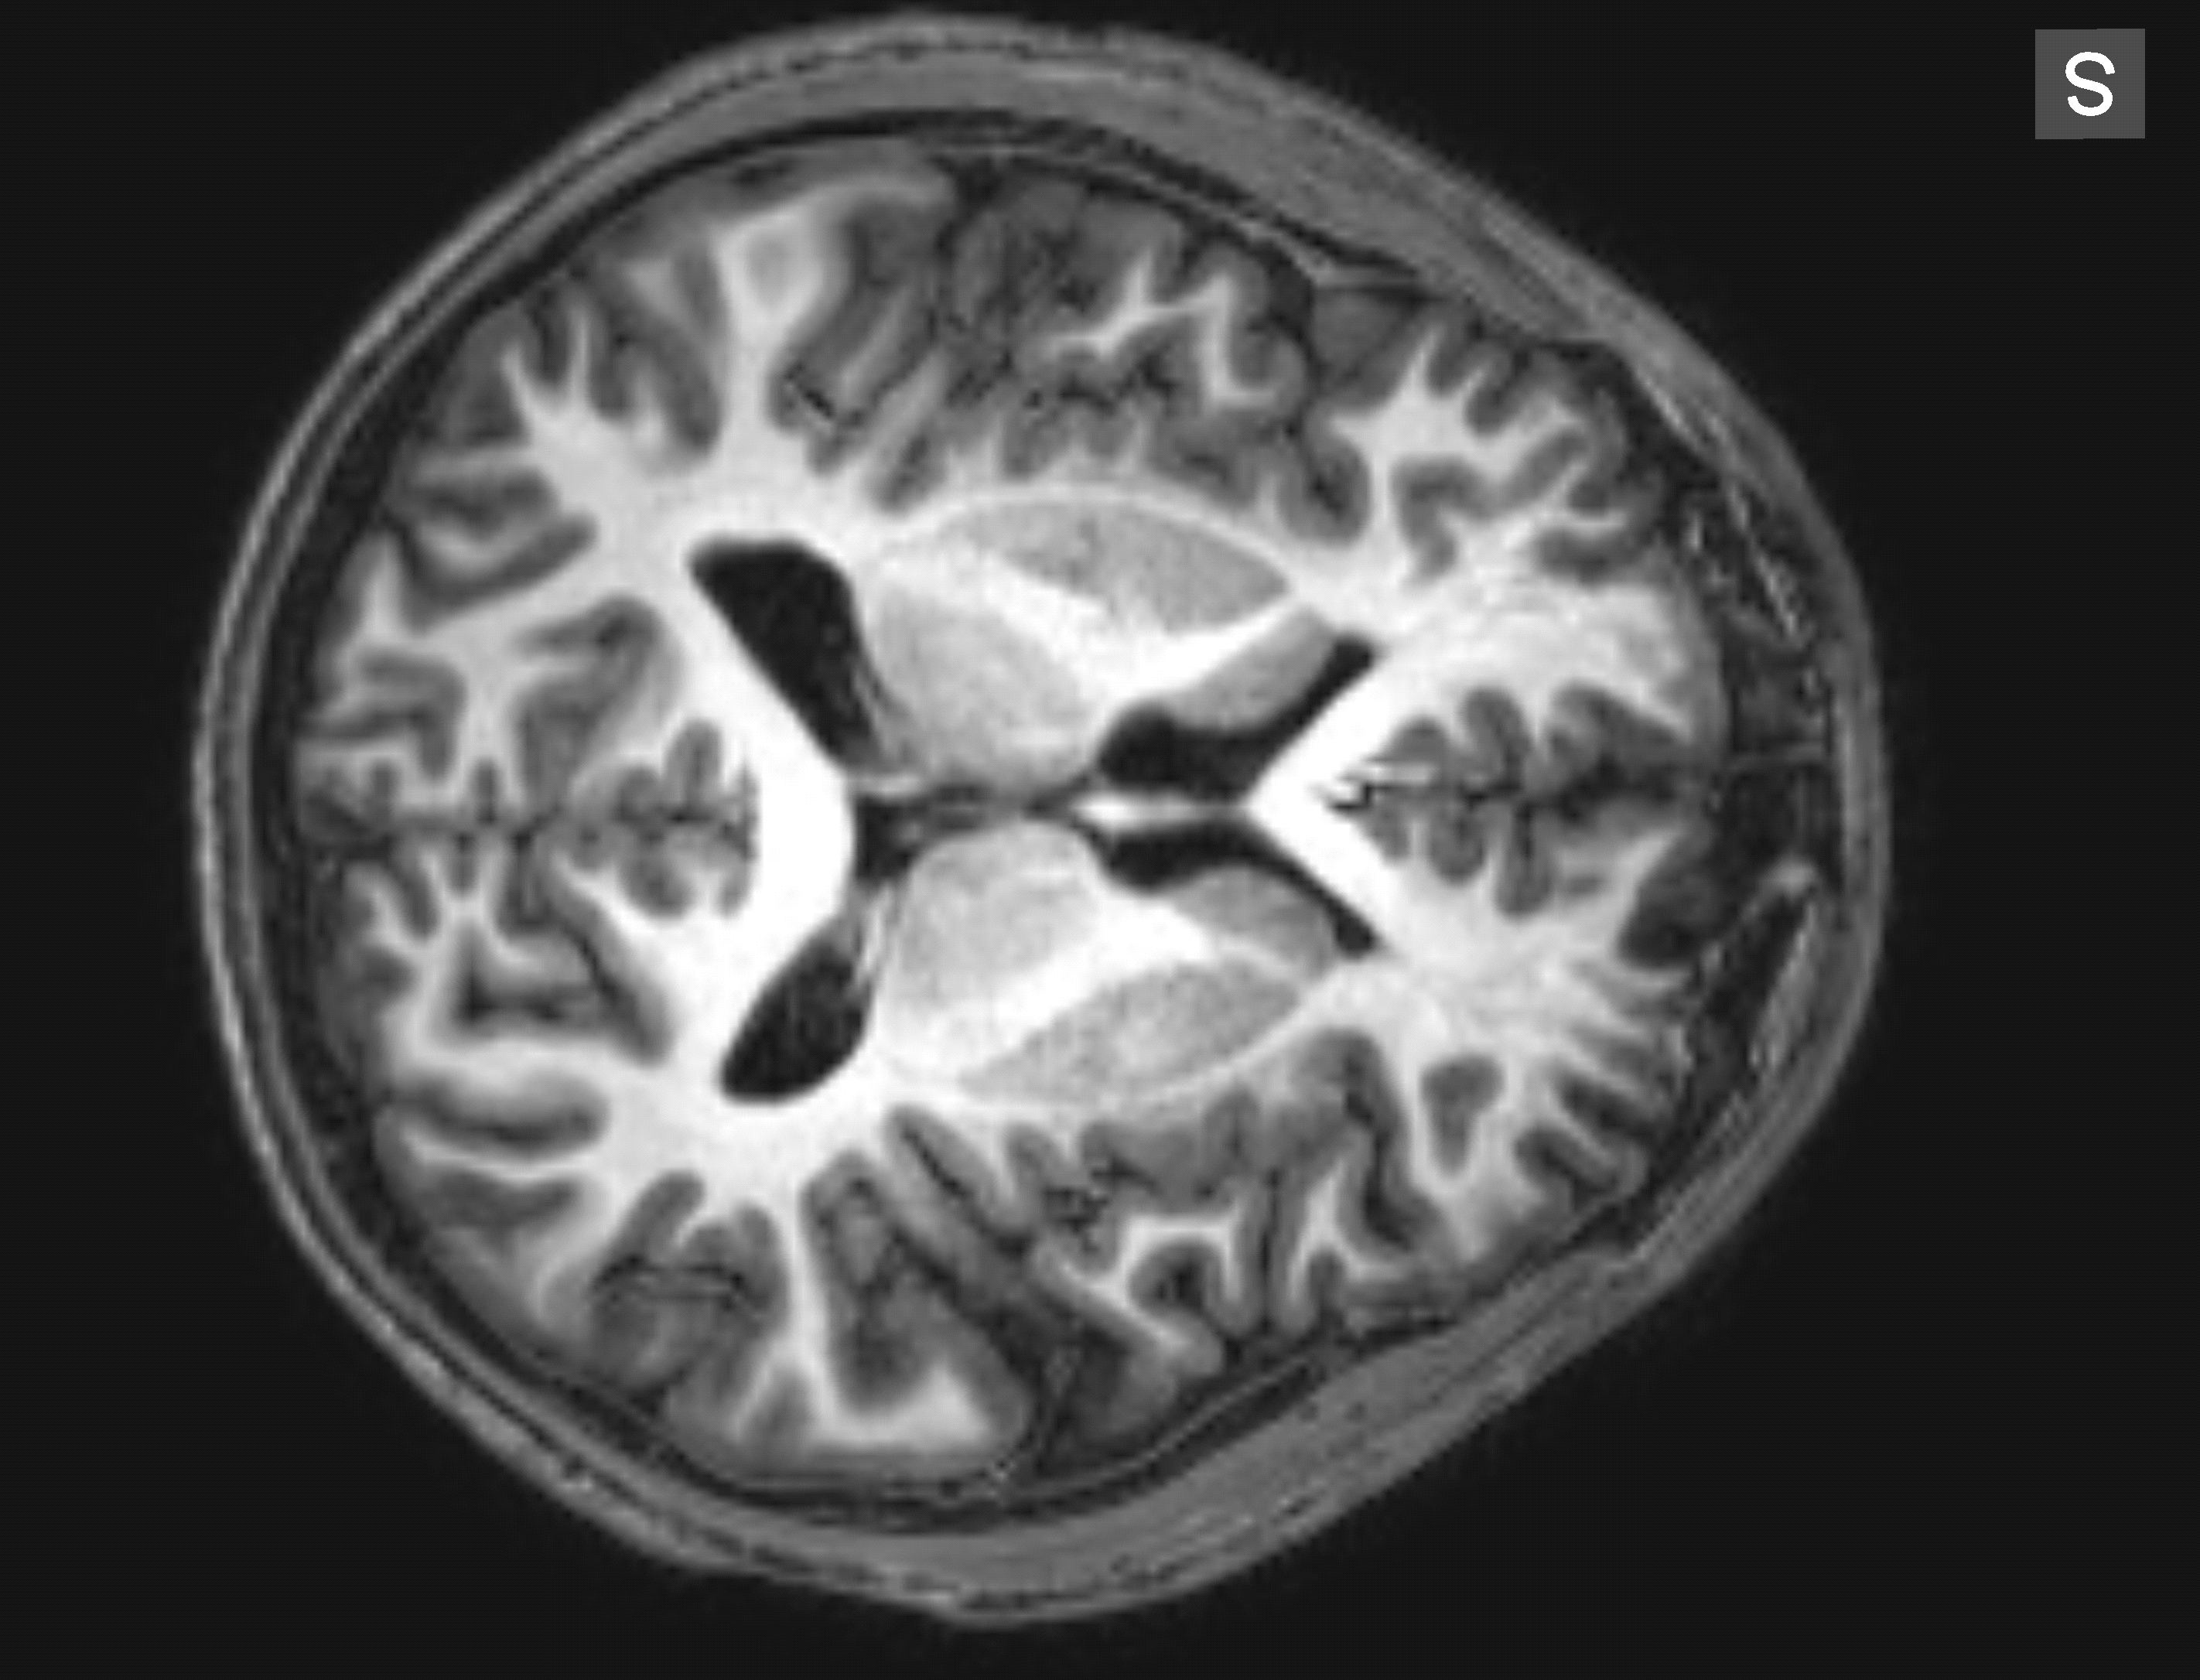
\includegraphics[width=\textwidth]{related/mri}
				\caption{T1}
    \end{subfigure} \hfill
		\begin{subfigure}{0.3\textwidth}
        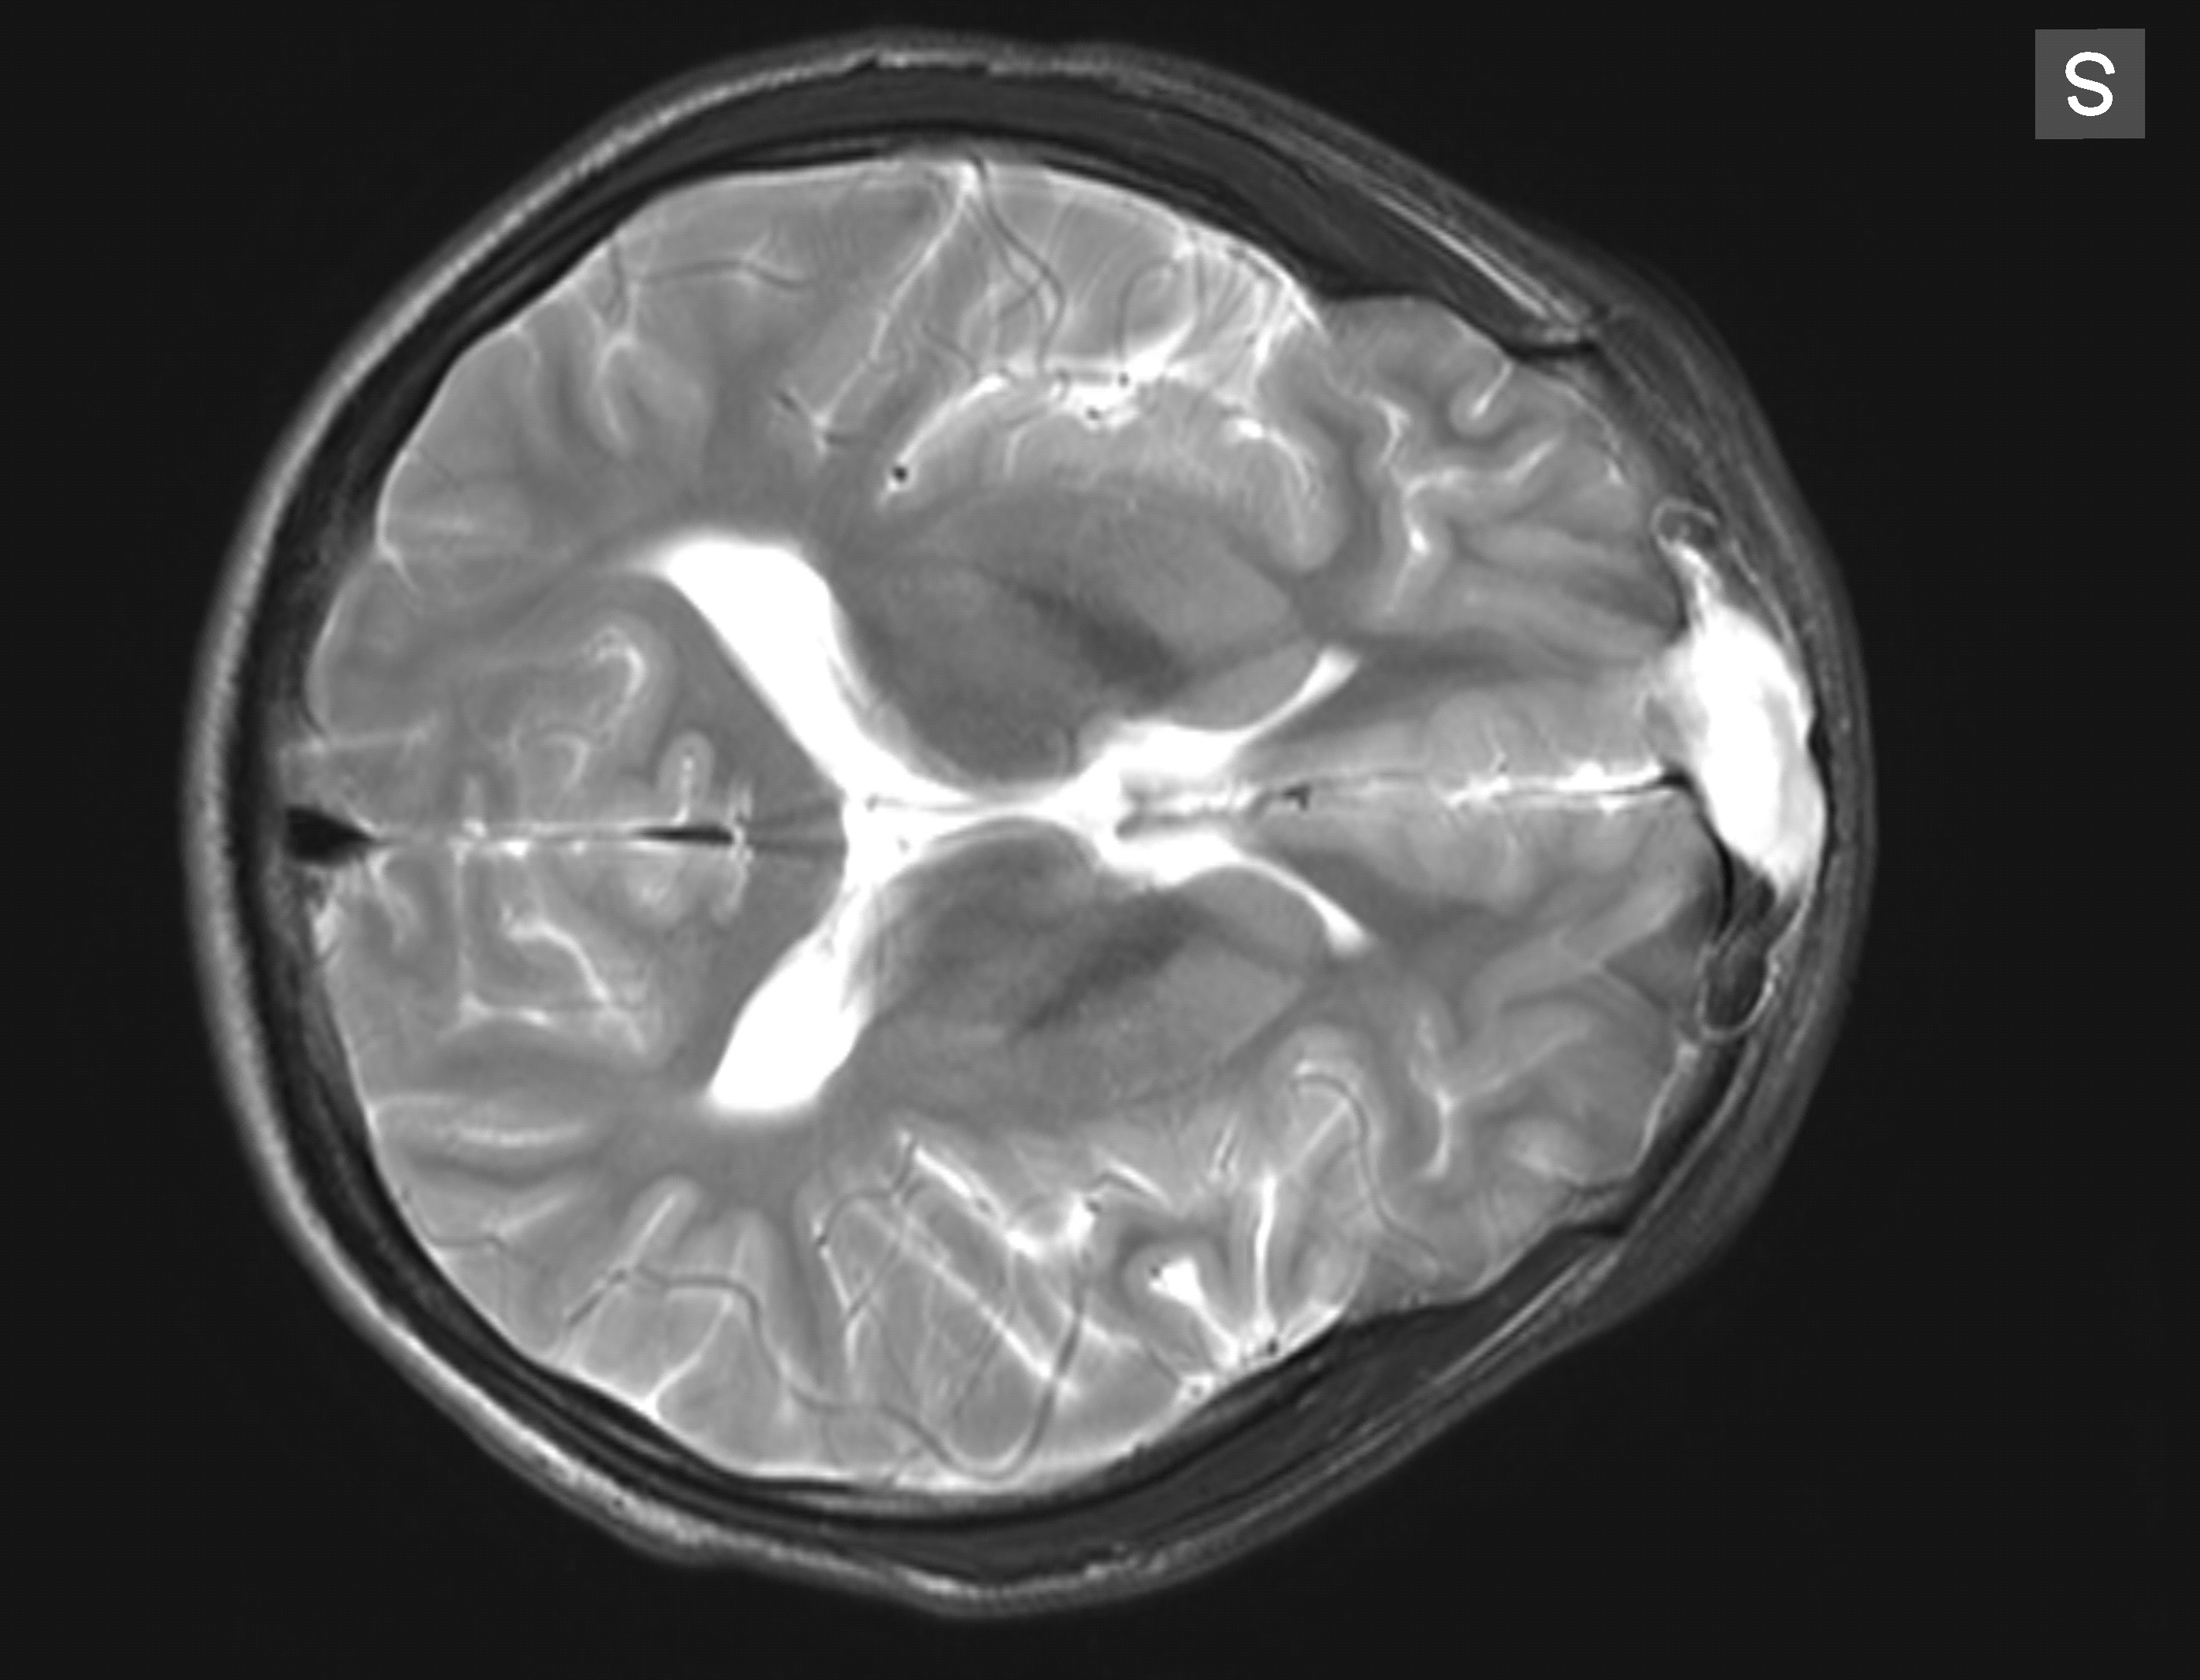
\includegraphics[width=\textwidth]{related/t2}
				\caption{T2}
    \end{subfigure} \hfill
		    \begin{subfigure}{0.3\textwidth}
        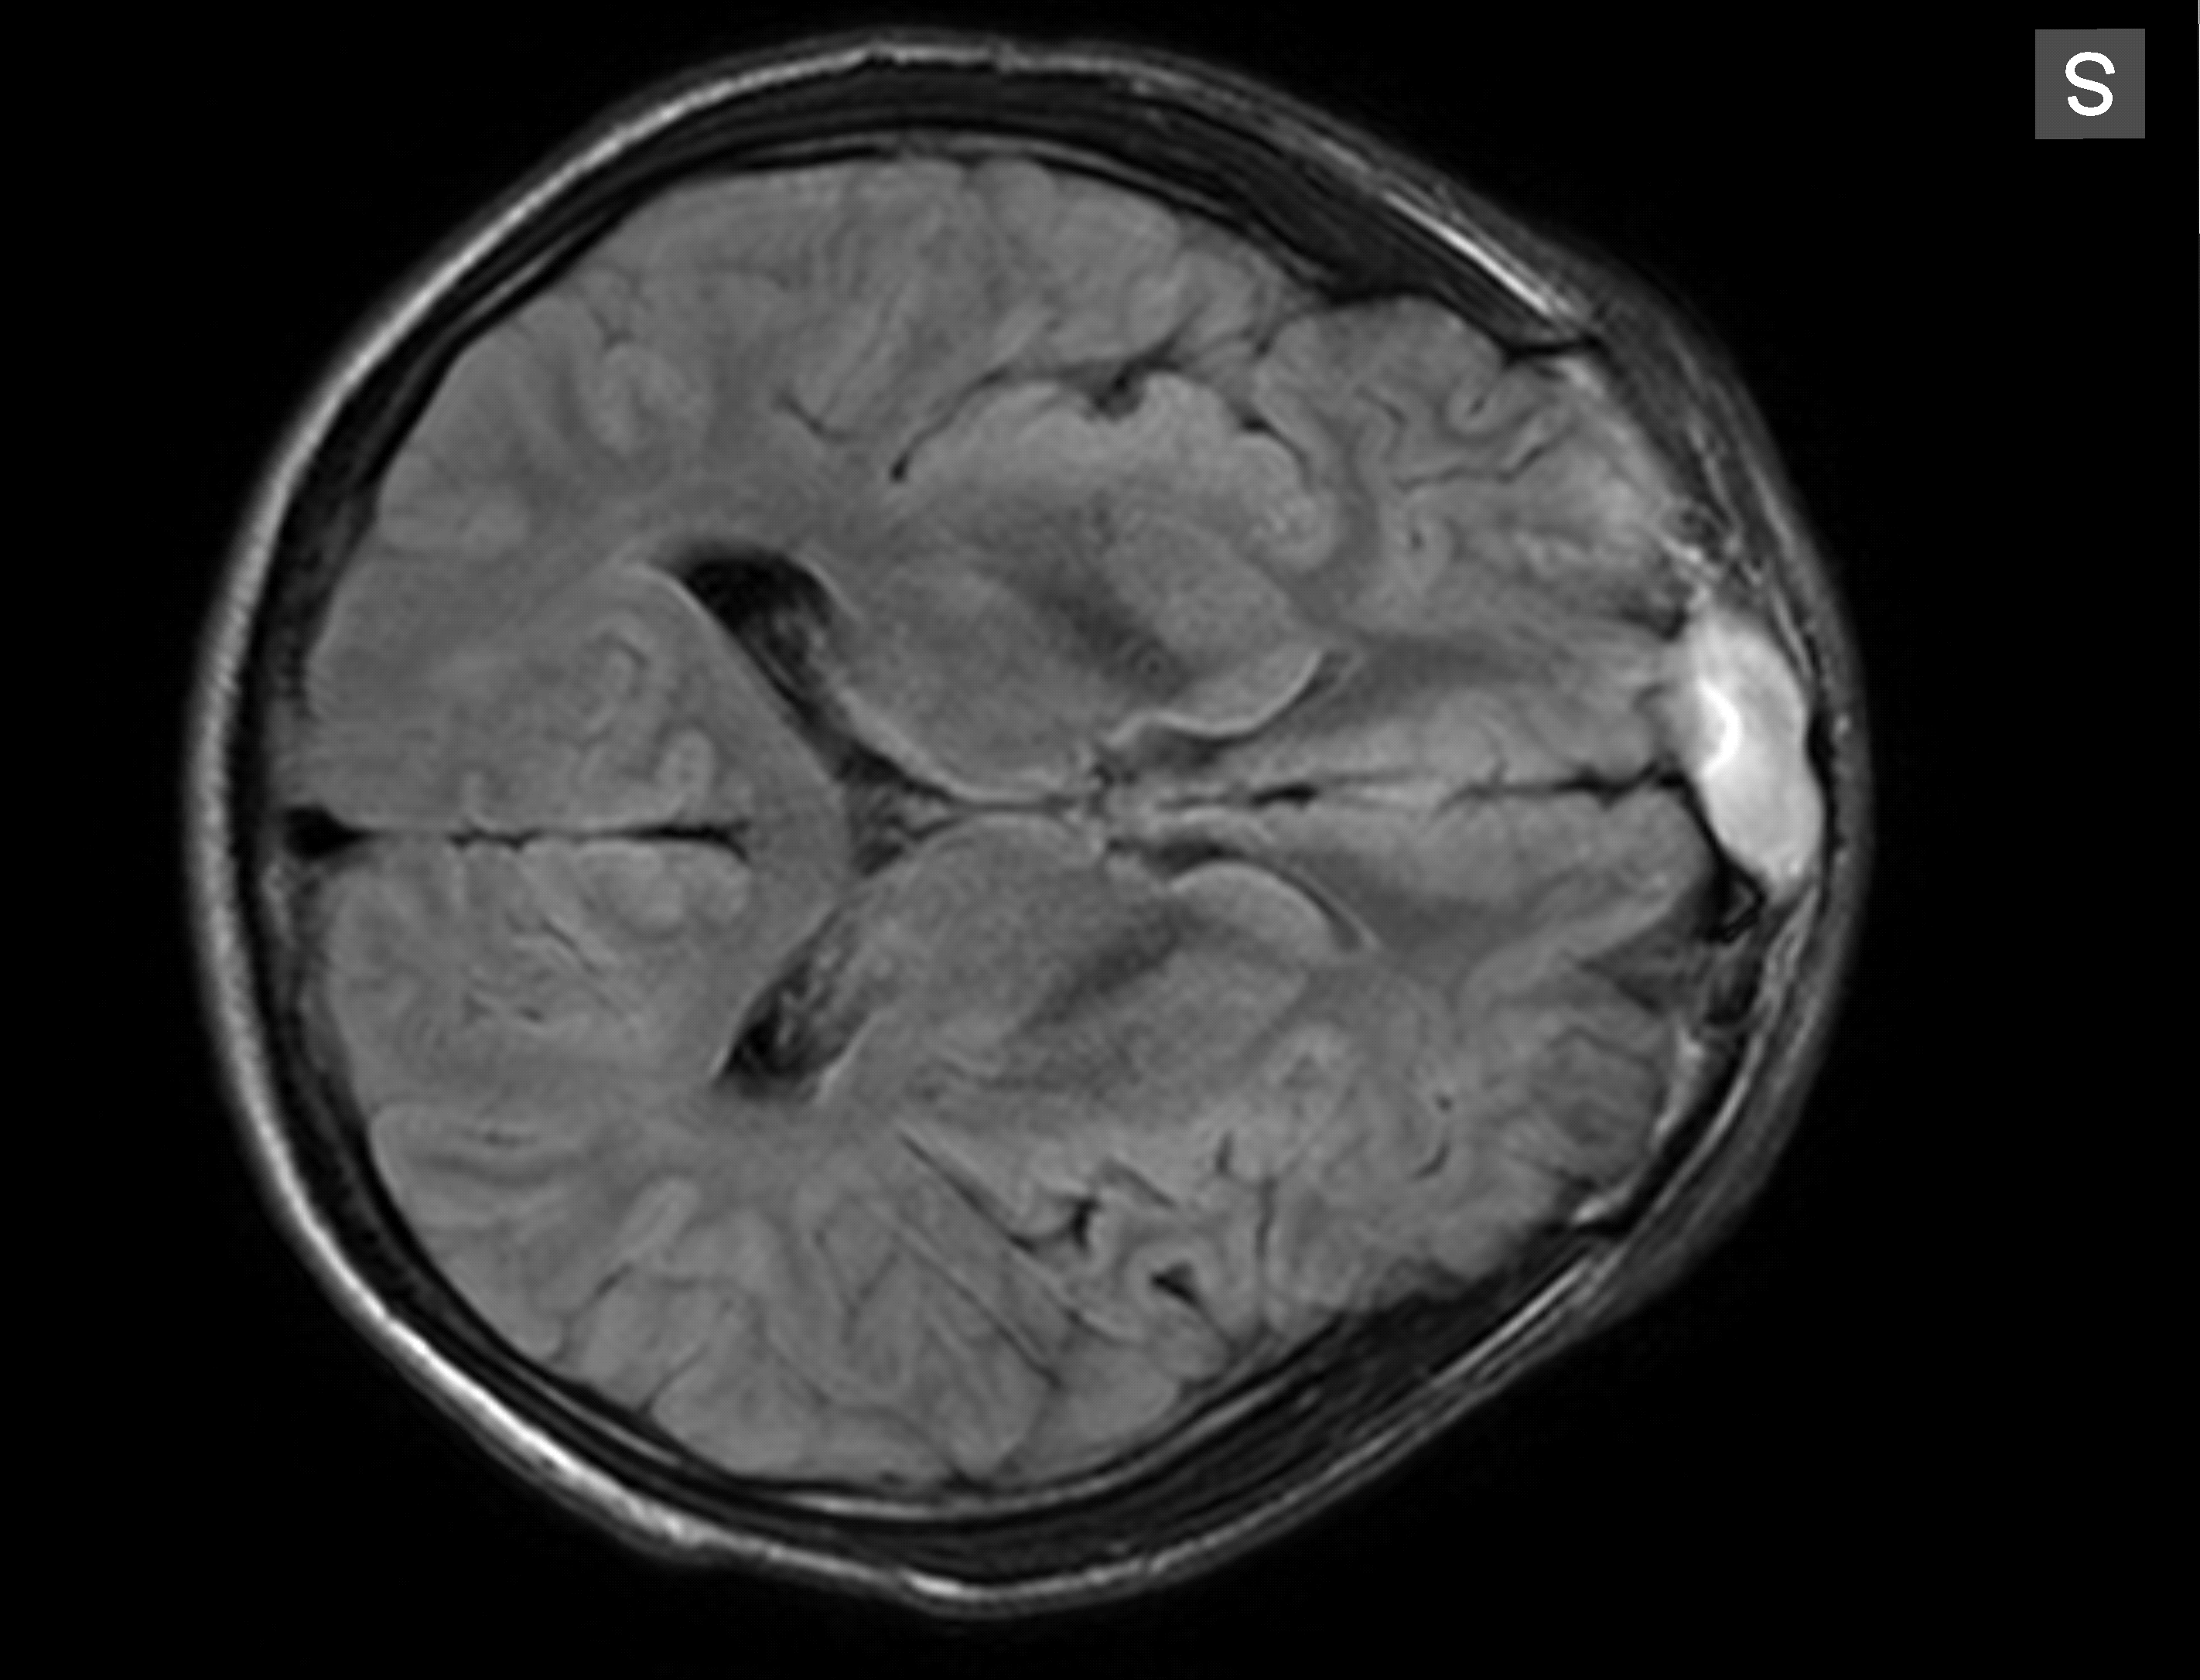
\includegraphics[width=\textwidth]{related/flair}
				\caption{Flair}
    \end{subfigure}
    \caption{Some MRI Contrasts}\label{fig_mri_mods}
\end{figure}

 
%Basics of images, voxels, coordinates, scalars

\subsection{Image Registration}

Neuro image data is usually represented as an array of voxels and an affine transformation. Usually structural images are represented as three dimensions arrays, while diffusion and functional images are series of three dimensional images or a four dimensions arrays. Elements in the array are numbered using integers, and the coordinates associated to the physical space of each voxel are obtained by applying the affine transformation to those integers. Distances in this physical space are associated to physical distances usually in mili-meters. The origin (zero) of this coordinate system may represent a meaningful location or may be arbitrary. 

Given two different images, it is likely they will use different coordinates systems. The most simple option is to estimate a third affine transformation that can map locations in one coordinate system to locations in the other. The estimation is usually iteratively, by minimizing a measure of disparity between both images. Software like FSL-FLIRT \autocite{jenkinson_fsl_2012} or SPM \autocite{friston_statistical_2007} can be used for this purpose. The affine transformations permits comparing locations at the two images, but the voxels coordinates will not match. If one wants to create a one to one match between voxels in one image to the other one, it is necessary to resample one of them. This process consist of interpolating the value of the scalars of one image at the locations of the desired voxel array. Resampling inevitably losses information, and therefore it should be done only when it is necessary.

Linear registration works well for images from different modalities or different sessions belonging to the same subject, as in this case displacements, rotations and scaling are enough to explain the differences. However, ``comparing two different brains is a challenging task, specially in the cortex where the pattern of folding between two subjects can be substantially different'' \autocite{toga_new_2002}. In this case, linear registration can still be applied and it will provide some very basic alignment. If done towards a reference brain (like \emph{Talairach} or \emph{MNI}), it will produce standard coordinates that can be used to report, share and compare results among researchers.

Non-linear registration methods provide a more powerful option to compare two different brains. These techniques use warp fields to distort the brain in different ways at different locations, and therefore can adjust to large topological differences. When the analysis involves a group of subjects, it is typical to first create a template brain representing the population, and then calculate warp fields between each subject and the template. Notice that these transformation must be invertible. Tools like ANTs, SPM or FSL can be used for this purpose (see \autocite{klein_evaluation_2009,klein_evaluation_2010}). Resampling can also be applied after non-linear registration, but in must be considered that the loss of information in this case is larger.
 
\subsection{Structural Images}

Structural images contain information about the anatomy of the brain and the elements that compose them. This category includes T1 and T2 weighted images, as well as fractional anisotropy (FA) and mean diffusion (MD) maps derived from DWI series. Segmentation is the process of dividing the image into the different structures or types of matter that make up the brain, gray matter, white matter and cerebro-spinal fluid (CSF). It can be done manually by image experts, or by using automatic algorithms. 

% SPM
% VBM

\subsubsection{Voxel Based Morphometry}

Voxel Based Morphometry (VBM) is a method that can be used to analyze differences in white or gray matter at each location of the brain \autocite{friston_statistical_2007}. For example, if one is interested in differences in gray matter between two groups in a study, the first step would be creating gray matter maps for every subject. Then the images would be co-registered to a template brain, and resampled. If one is interested in global gray matter differences then resampling must be done in such a way that the total volume of gray matter is conserved. Next, a Gaussian filter of appropriate width (depends on the expected size of the differences under analysis) is applied to all images. Finally, a statistical model is fit at every voxel using the group labels as regressors and the amount of gray matter as outcome. The final output will be a statistical map, where locations with a large difference of gray matter between the two groups will have high values. 

% Segmentation of hippocampus, robust in presence of pathology \autocite{kim_robust_2011}.

\subsubsection{Automatic Segmentation}

FreeSurfer \autocite{dale_cortical_1999-1, fischl_whole_2002} is a software package which can perform automatic segmentation of sub-cortical brain structures, cortical surface reconstruction and cortical parcellation; as shown in Figure \ref{fig_fs_out}. Cortical surfaces from different subjects are also mapped to a standard cortex, which allows researchers to compare cortical thickness (and other scalars) between subjects along the cortex. The software also reports the volumes of all sub-cortical structures, which can be used in classical statistical analyzes. The project presented in this thesis makes heavy use of FreeSurfer's results.

\begin{figure}
    \centering
    \begin{subfigure}{0.3\textwidth}
        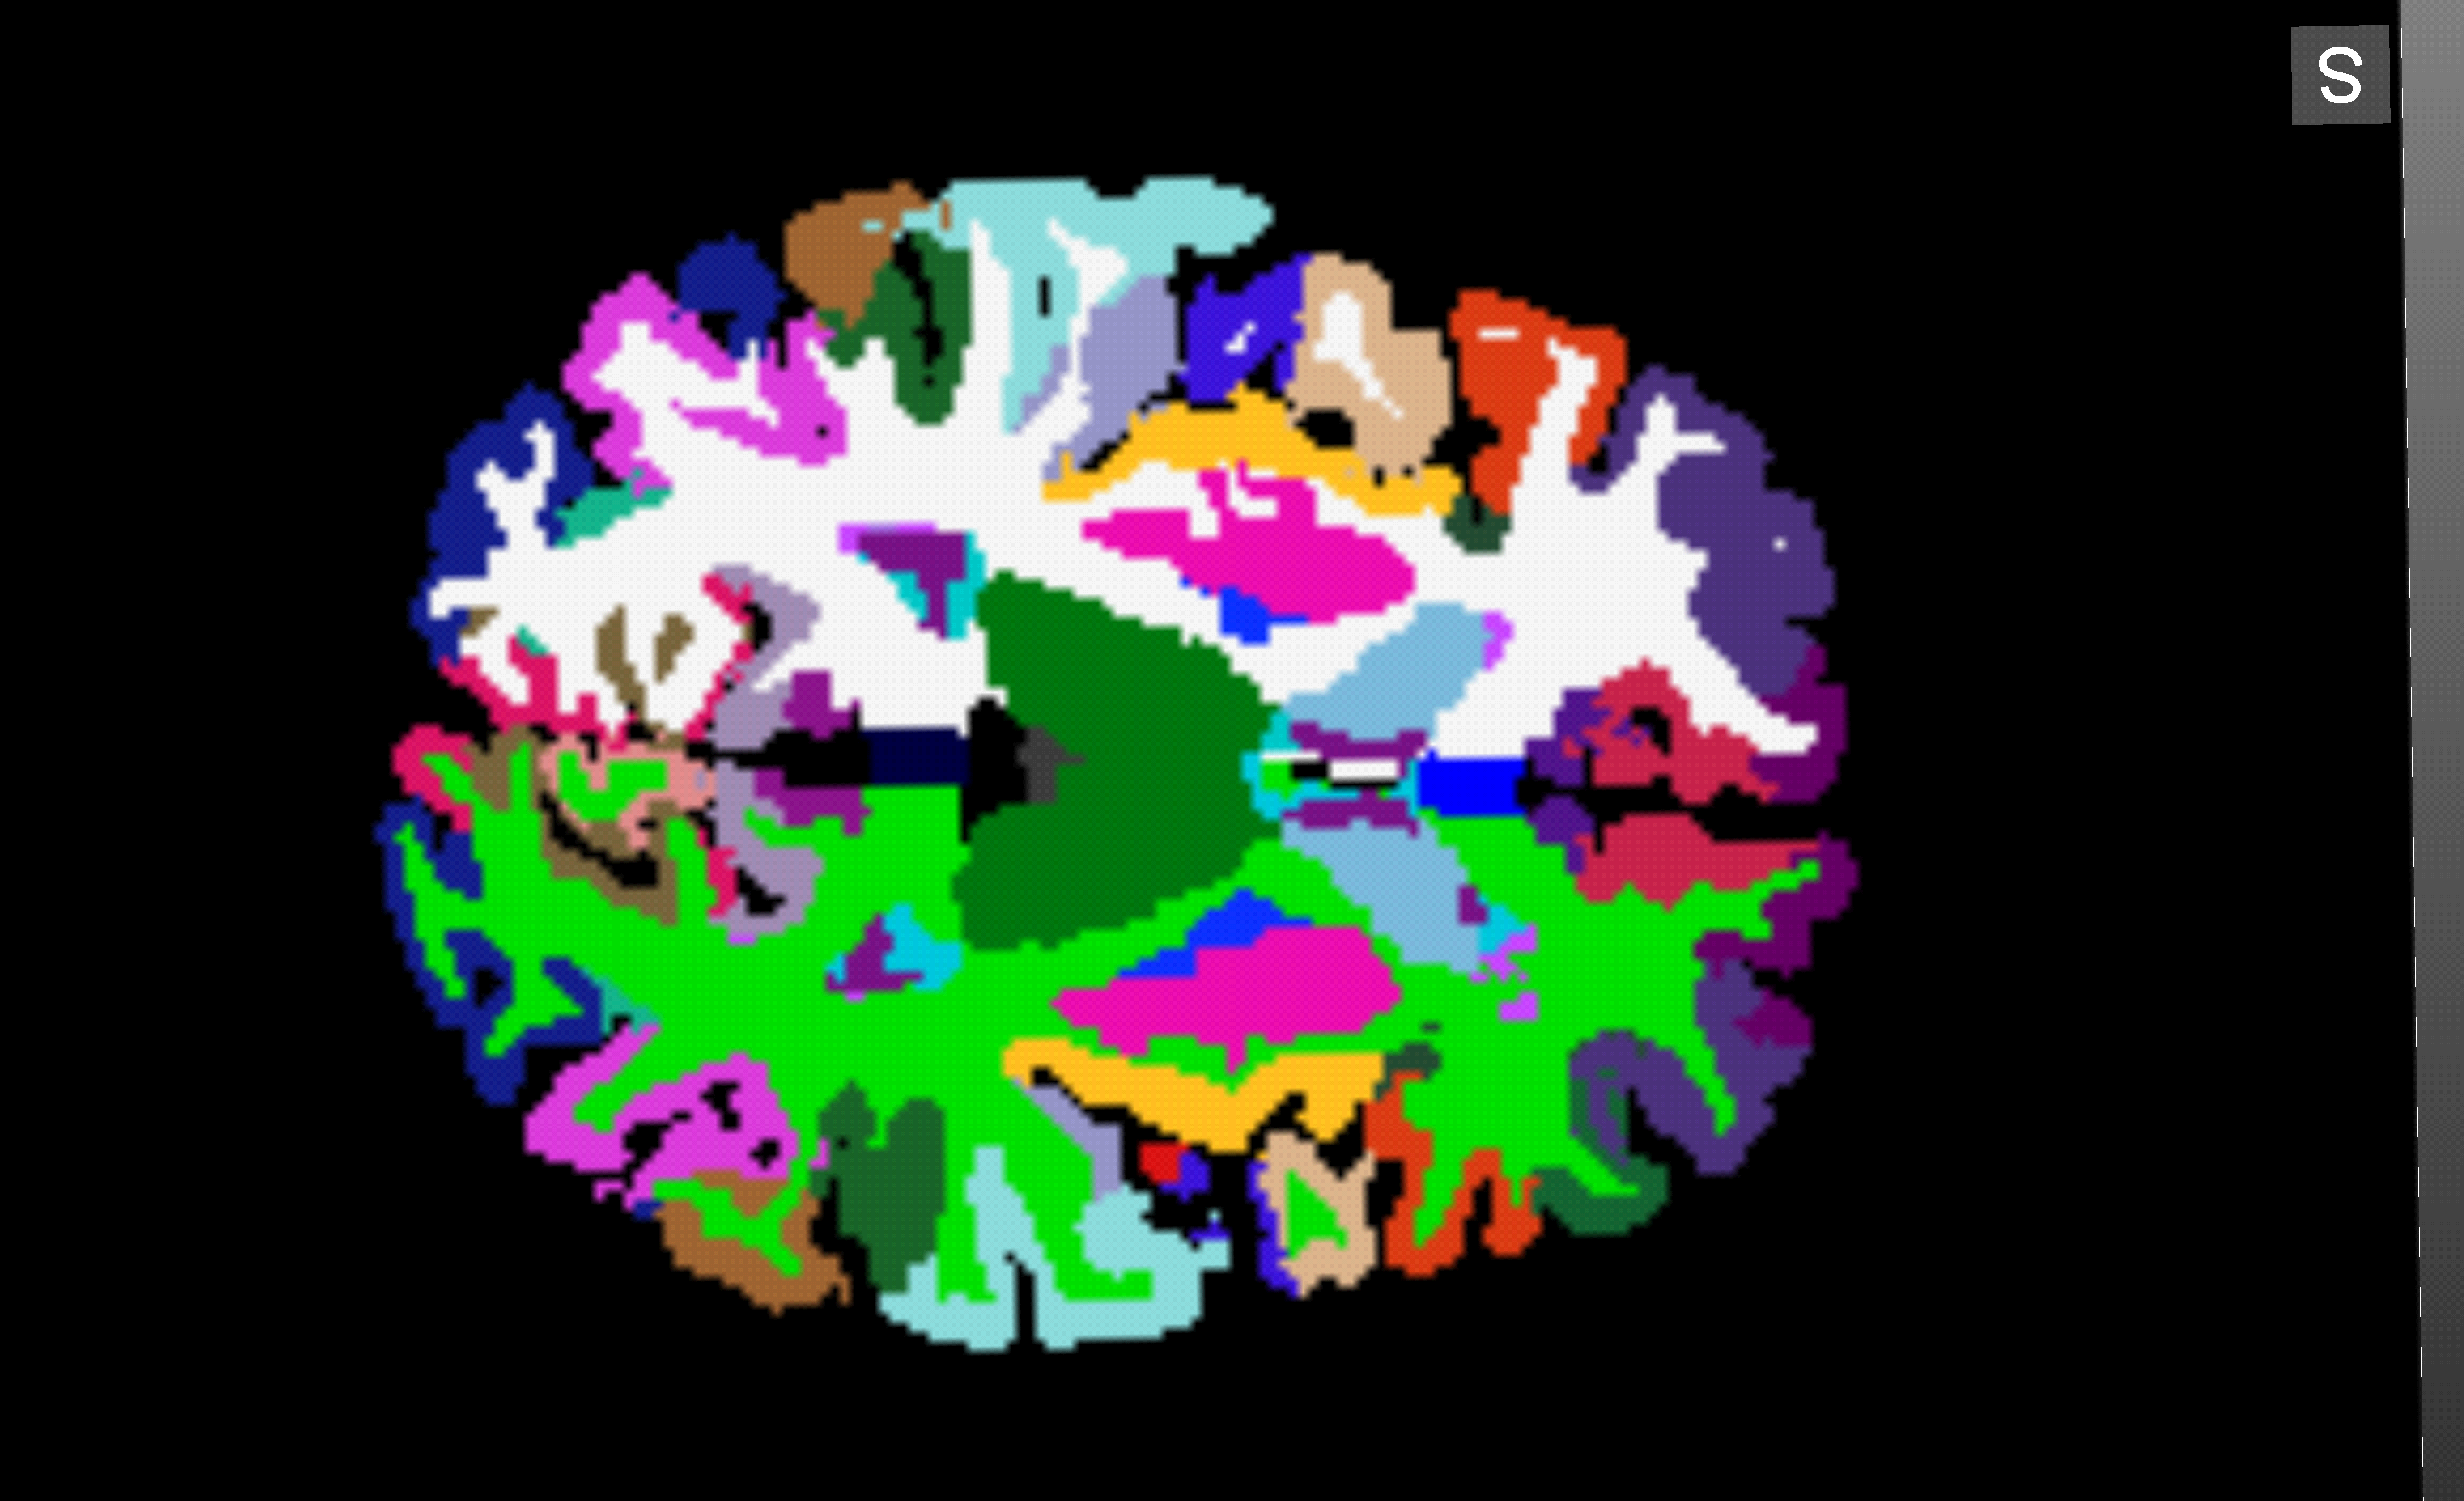
\includegraphics[width=\textwidth]{related/aparc}
				\caption{Segmentation}
    \end{subfigure} \hfill
		\begin{subfigure}{0.3\textwidth}
        \includegraphics[width=\textwidth]{related/surf_thick}
				\caption{Cortical Thickness}
    \end{subfigure} \hfill
		    \begin{subfigure}{0.3\textwidth}
        \includegraphics[width=\textwidth]{related/surf_parc}
				\caption{Cortical Parcellation}
    \end{subfigure}
    \caption{Free Surfer Output}\label{fig_fs_out}
\end{figure}

\subsubsection{Shape Analysis}

Segmented structures can be reconstructed and used for shape analysis, this is, analyzing differences in the whole shape of a structure. 
Spharm \autocite{gerig_shape_2001} is a method that parametrizes shapes, and can then statistically compare the shapes of different subjects across all points.  \autocite{hermann_visual_2014} propose a system to interactively explore shape variations between a structure from different subjects or at different times. The system provides three different visualizations at different levels of detail. The first view shows the overall pattern across the structure, the second one allows the user to focus on a substructure and see how changes on it are related to the rest of the structure, and the final one lets the user interactively modify the structure by dragging a  point and see how the rest of the structure would be modified. 

\subsection{Functional Magnetic Resonance}

In fMRI several BOLD volumes are acquired through the duration of the experiment. In the mean time the subject may be performing a task, reacting to stimuli or in resting state. During the course of the experiment the subject's head may move some mili-meters, therefore the first step in the processing pipeline is performing a spatial realignment of all the volumes. After this step there will be a timeline associated with each voxel. Some authors recommend applying a Gaussian filter at this stage (\autocite{friston_statistical_2007}) while others don't (\autocite{goebel_brainvoyagerpast_2012}). One possible analysis is searching for correlations between the signals at different voxels, and from them inferring which regions are connected. A possible outcome is a correlation map where voxels associated to a certain region have a strong signal. Another option is constructing a graph where nodes are regions and links are weighted by the correlation of the signals between them. Note that these correlations may change during the course of the experiments \autocite{richiardi_decoding_2011}. The analysis of this class of graphs will be discussed later with similar graphs derived from DWI. 

Another more traditional analysis option consists on explaining the BOLD signal using the experiment design (stimulus or task) as a regressor, possibly considering also other confounders (for example the estimated motion of the head). The experimental design should be convoluted with an hemodinamic response function that explains the delay between a stimulus and the associated increase in oxygen (see \autocite{poldrack_handbook_2011}). After fitting the statistical model at each voxel, statistical maps can be generated for each contrast, where a contrast is a combination of the conditions or factors that make up the experiment. For example, if an experiment interleaves actions with the left and right hands, possible contrasts could be the effect of the left hand, the effect of the right hand, or the difference between both hands. This statistical maps will contain high values for regions where the BOLD signal can be well explained by the contrast. There will be such a map for each subject.

A second level analysis can then be done to compare the maps of different subjects, and use linear models to explain the differences based on some other variable. The method for this analysis is similar to VBM. 

These analyzes can be carried out using SPM \autocite{friston_statistical_2007}, AFNI \autocite{cox_afni:_1996}, Brain Voyager \autocite{goebel_brainvoyagerpast_2012} and FSL \autocite{jenkinson_fsl_2012} among others \autocite{gold_functional_1998}.

%BrainVoyager \autocite{goebel_brainvoyagerpast_2012} is a commercial package for high performance processing of functional, diffusion and structural brain data. Its algorithms are optimized for producing fast results (some even realtime), by using all of the available hardware. It includes a scripting language for analyzing bulks of images, and it is also incorporating the newest techniques as Multi-Voxel pattern analysis, a machine learning technique for inferring the state of the mind based on data from functional imaging and a previous training. By doing this analysis in real time it can be used for brain computer interfaces. 

\subsection{Diffusion Weighted Images}

% acquisition
% HARDI

During a DWI protocol several volumes are acquired using a signal that is sensible to water diffusion in a given direction (see \autocite{jellison_diffusion_2004} for more details). Typically around thirty volumes are acquired in different directions, but a new technique known as high angular resolution diffusion imaging (HARDI) uses hundreds of directions. One or more images without any diffusion gradient are also acquired in the series to use as anatomical reference, this images have a contrast similar to T2 weighted images.

% modeling
% tensors and more
Processing of DWI begins by realigning the volumes and correcting for known noise sources. The next step is estimating a diffusion model on each voxel, based on data for the different directions. Frequently a tensor model is used, which represents diffusion of a voxel as a tensor, this technique is called diffusion tensor imaging (DTI). This model has six degrees of freedom, and is adequate for discrimating between regions where diffusion is isotropic (CSF and grey matter), and regions where diffusion is predominant in one direction (similarly oriented myelinated axons). However this model fails when there are crossing fibers, or fibers that bend in tight angles. Also, compressing the information from hundreds of volumes in just six degrees of freedom causes an important loss of information. In the recent years more complex models that solve these problems have been developed \autocite{tournier_diffusion_2011}.  

% scalars, fa and more
From these diffusion models several scalar values can be derived. One of them is the fraction of anisotropy (FA), which goes from zero to one, and represents how directed is the diffuion on a given voxel. This value is usually associated to the amount of myelin present in brain fibers. Another interesting value is the mean diffusion (MD) which measures the total amount of diffusion going on at each voxel (see Figure \ref{fig_dwi_scalars}). This value will be high on areas with large amounts of water, for example the ventricles. FA images can be compared among subjects using techniques similar to VBM. TBSS \autocite{smith_tract-based_2006} is another approach, characterized by a co-registration based on the main white matter pathways

\begin{figure}
    \centering
    \begin{subfigure}{0.3\textwidth}
        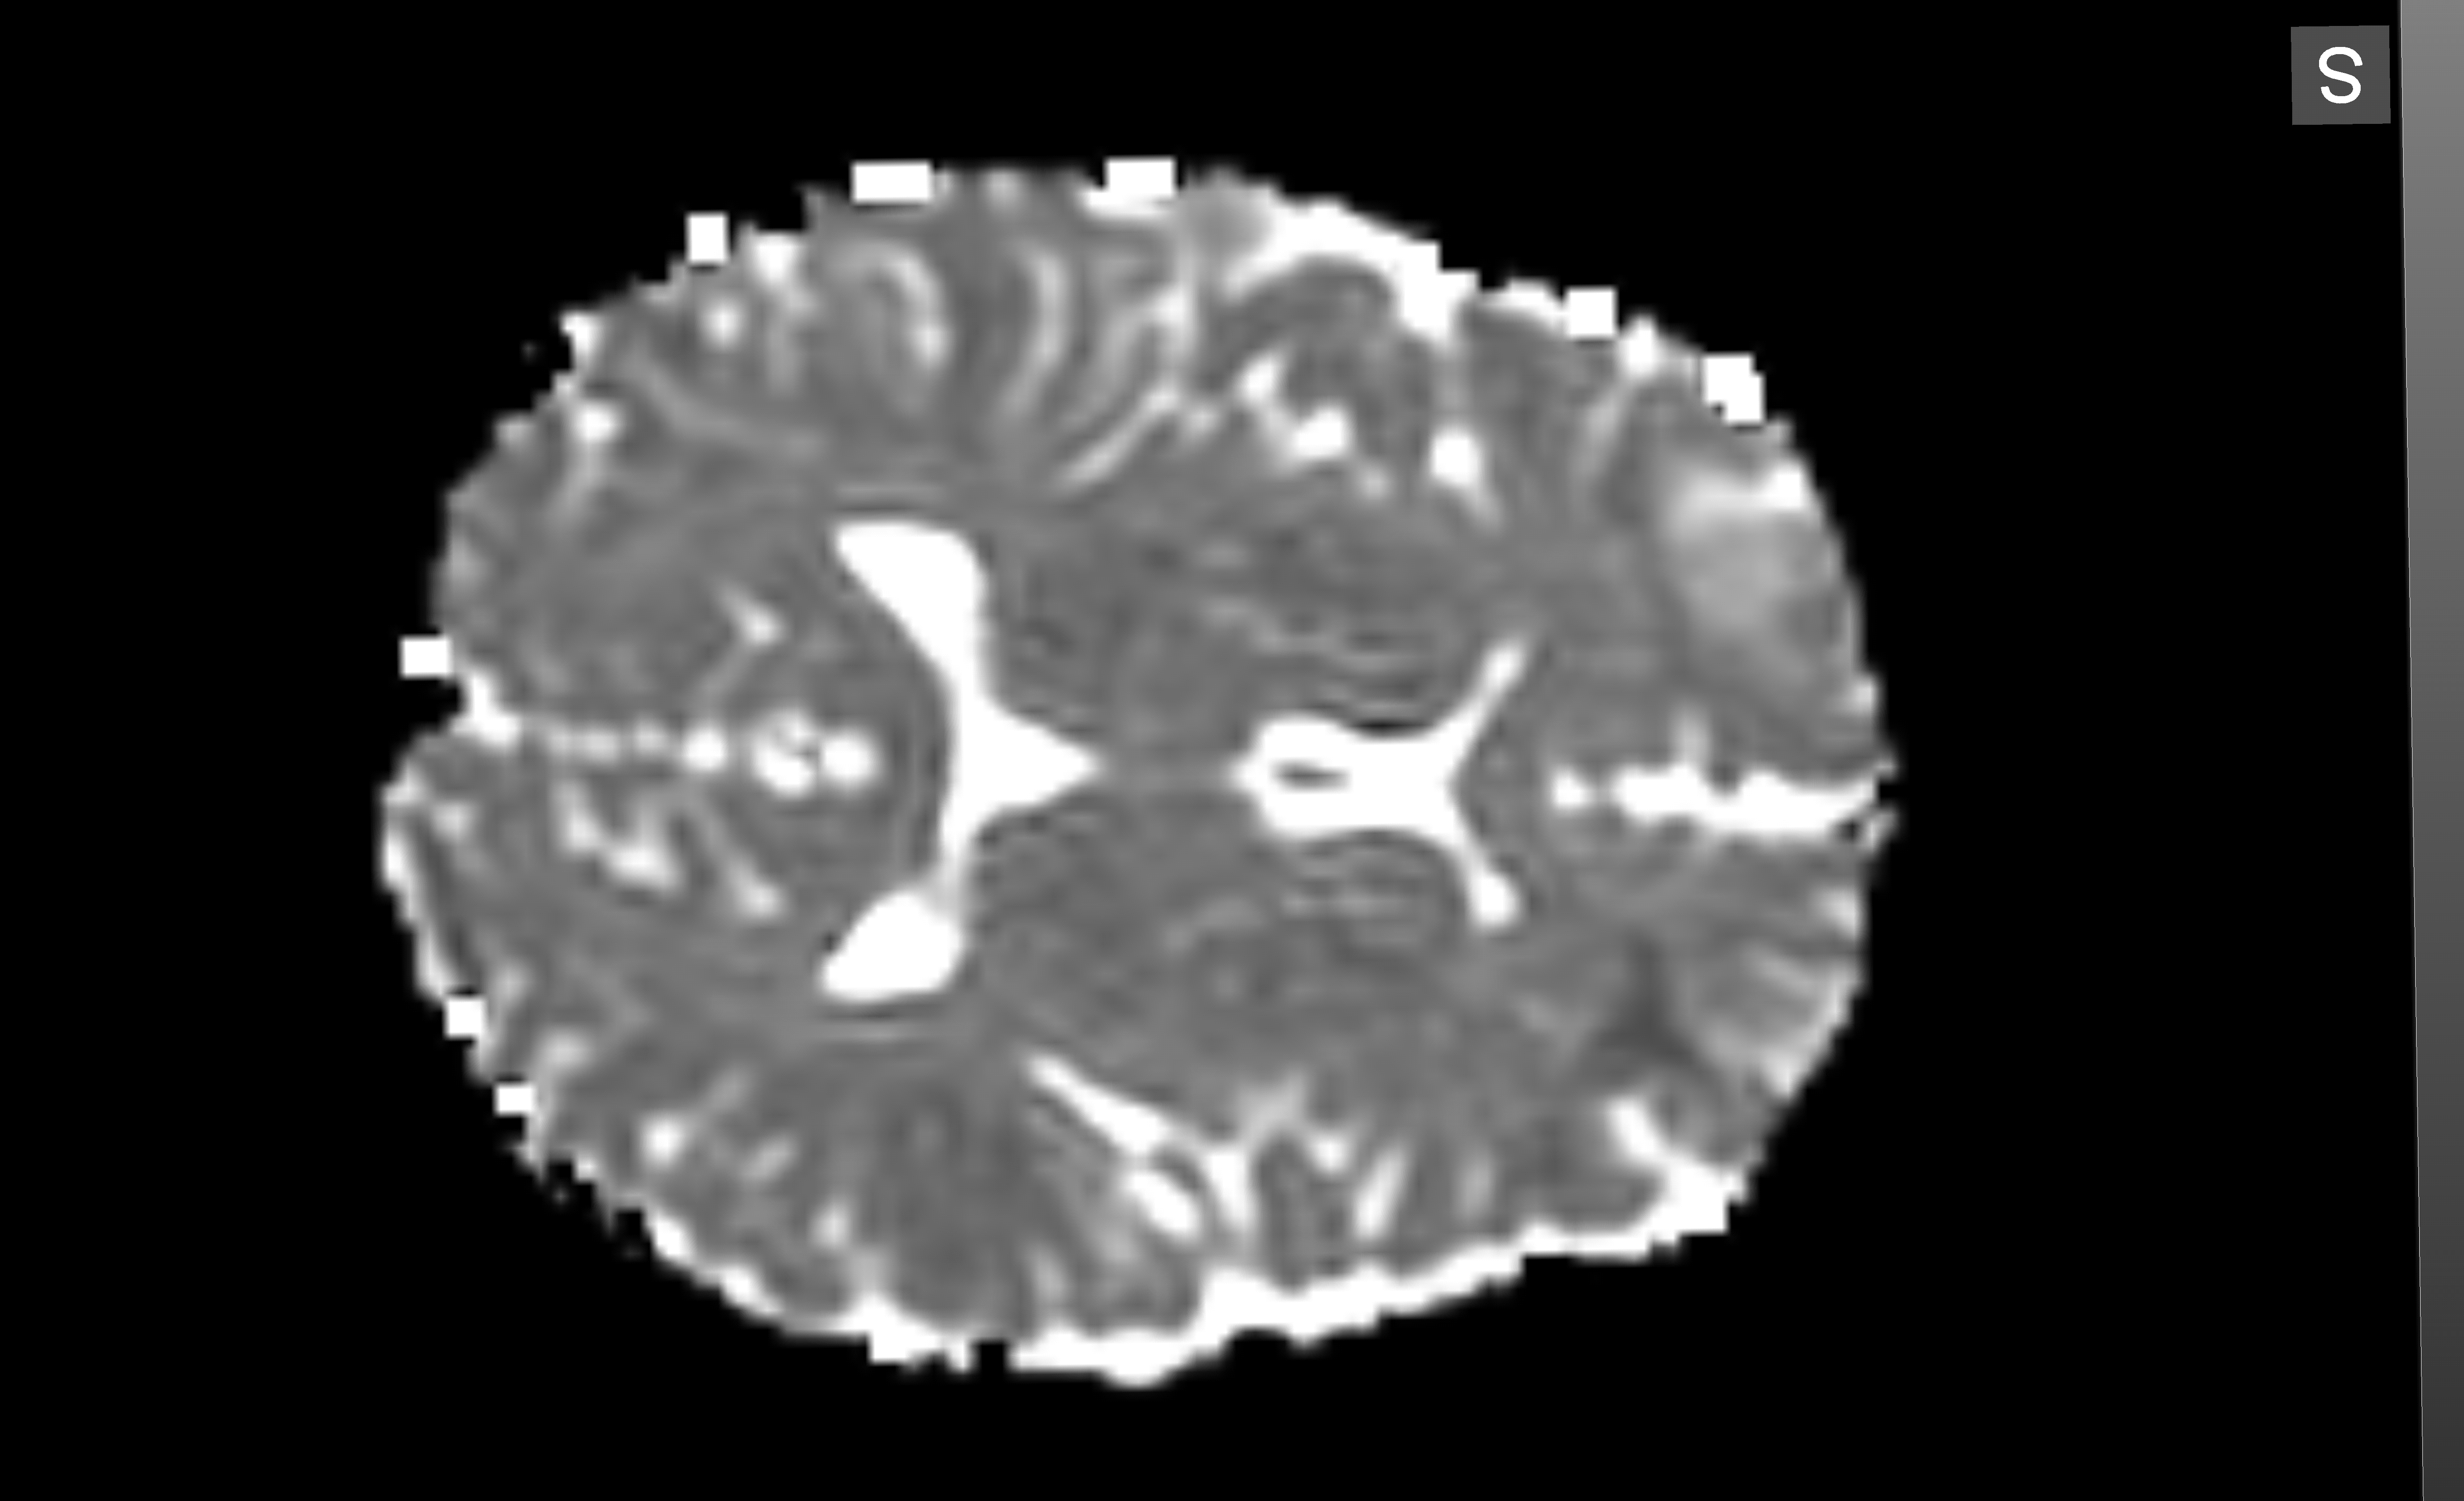
\includegraphics[width=\textwidth]{related/md}
				\caption{MD}
    \end{subfigure} \hfill
		\begin{subfigure}{0.3\textwidth}
        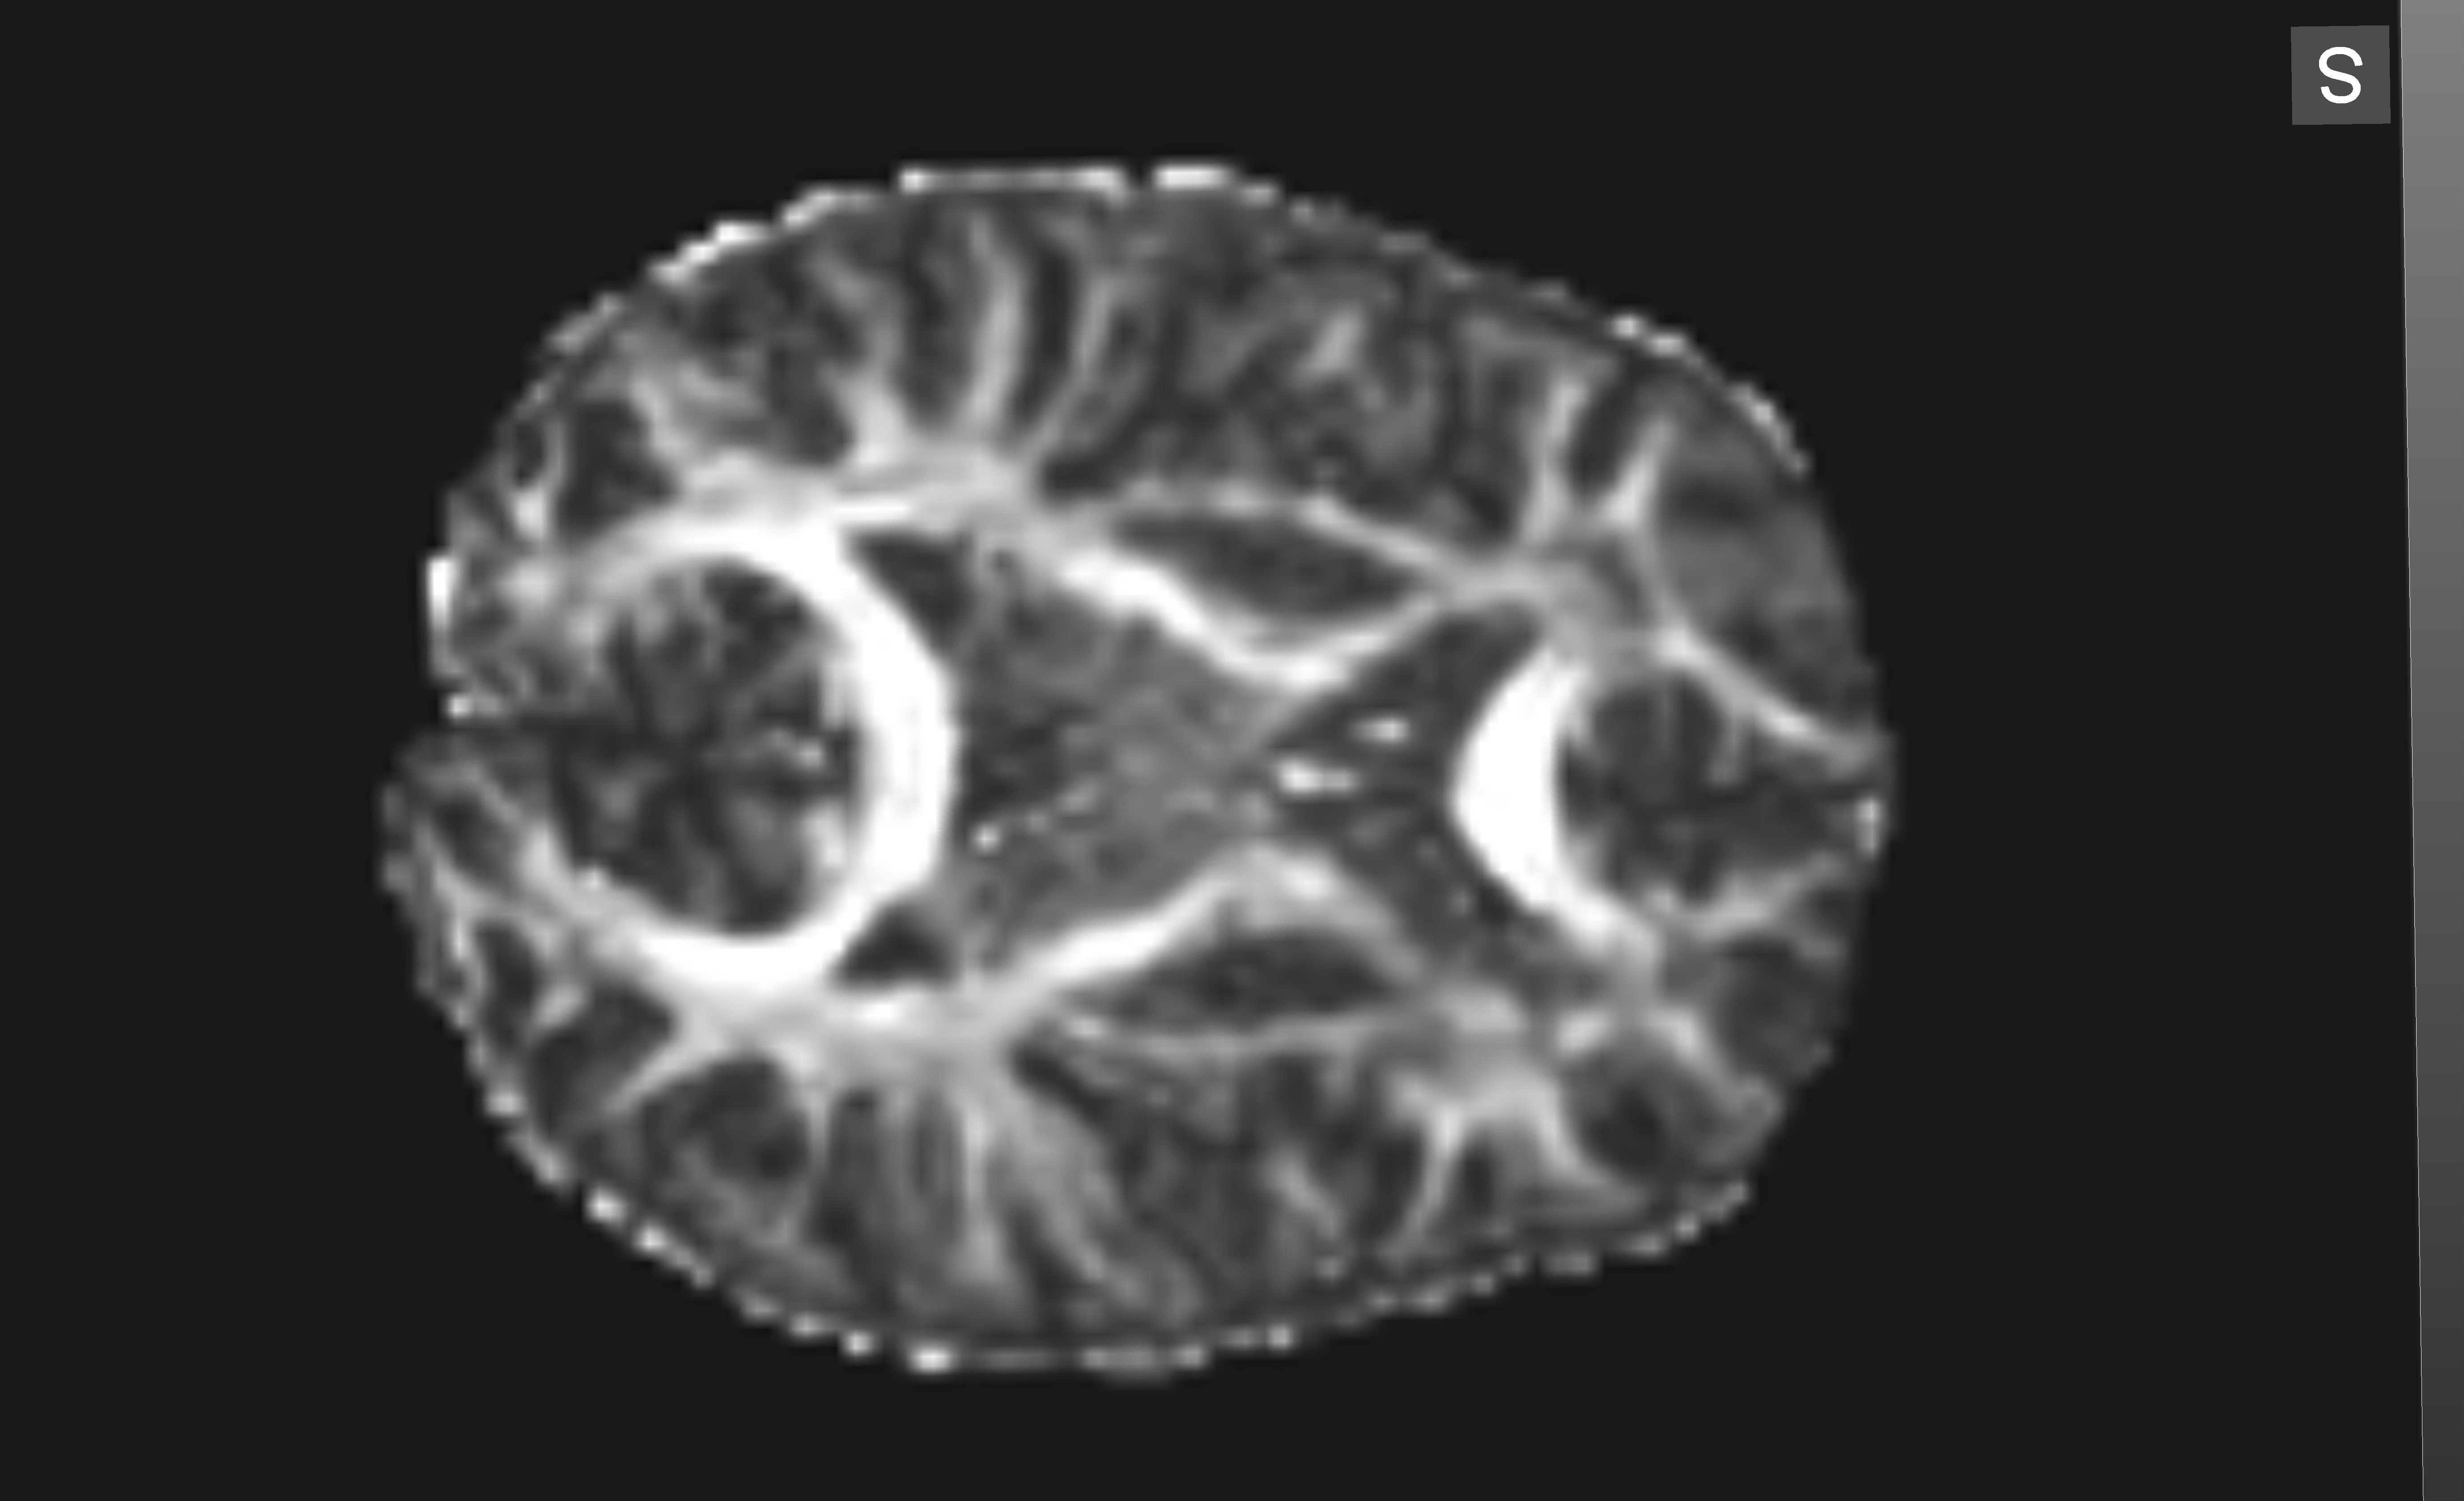
\includegraphics[width=\textwidth]{related/fa}
				\caption{FA}
    \end{subfigure} \hfill
		    \begin{subfigure}{0.3\textwidth}
        \includegraphics[width=\textwidth]{related/dti}
				\caption{Color DTI}
    \end{subfigure}
    \caption{DTI scalars and color representation}\label{fig_dwi_scalars}
\end{figure}


\subsubsection{Tractography}

% tracking
After the diffusion model for every voxel is available, it can be used to generate streamlines that represent full brain fibers. This technique is called tractography, and the basic algorithm starts each line at specific seed points, and then propagates them along the main diffusion direction of each voxel; but several enhancements and variations have been developed. The newest algorithms are probabilistic \autocite{behrens_probabilistic_2007} and provide output as likelihood maps (see Figure \ref{fig_tracto_det_prob}).
Reconstructing fibers that cross each other, or fold in tight angles is a hard problem \autocite{fillard_quantitative_2011}, and specially tensor based methods are not able to deal with them \autocite{tournier_diffusion_2011}. 

Algorithms for processing diffusion data are available in several packages, such as camino \autocite{cook_camino:_2006}, dipy \autocite{garyfallidis_dipy_2014}, dti studio \autocite{jiang_dtistudio:_2006} and diffusion toolkit \autocite{wang_diffusion_2007}
(see \autocite{hasan_review_2011} for a full review). 
Tracula \autocite{yendiki_probabilistic_2008} is part of the FreeSurfer suit, and it is especial because it uses anatomical priors together with diffusion data to estimate the most likely paths for the main brain pathways.

% bundles selection

Tractographies provide visual information about white matter structure in a particular subject and  is useful for planning surgeries as it indicates the positions of principal tracts. However full brain tractographies are usually very crowded, and they must be filtered to allow analysis. 
For example \autocite{blaas_fast_2005} presents a method for isolating fiber bundles by defining several regions of interest. Internally bundles are organized in a KD-Tree which permits interactive selection. 

% scalars among fibers

For research purposes it is important to compare tractographies from different subjects. The usual pattern is isolating pathaways of interest, either manually by placing regions of interest or using automatic atlas based methods, and then calculating the mean FA in the bundle, the mean length, the mean MD or the mean length. This scalar values can then be used on statistical methods.
\autocite{goodlett_group_2008} proposes a method for performing statistical analysis of white matter, by constructing a representative fiber bundle of the population under study, mapping it back to the diffusion image of each subject and sampling scalar values from it. In this way statistics can be performed along the tract, with scalars taken equivalent locations on each subject. In \autocite{colby_along-tract_2011} a different method for doing this is presented. Here fiber bundles are isolated on each subject using any method, and then each fiber in the bundle is resampled to a standard number of points. Scalar values are aggregated into this points. Statistical methods can then be used for each of this points, and also across subjects.

\begin{figure}
    \centering
    \begin{subfigure}{0.48\textwidth}
        \includegraphics[width=\textwidth]{related/tractography}
				\caption{Deterministic Tractography}
    \end{subfigure} \hfill
		\begin{subfigure}{0.48\textwidth}
        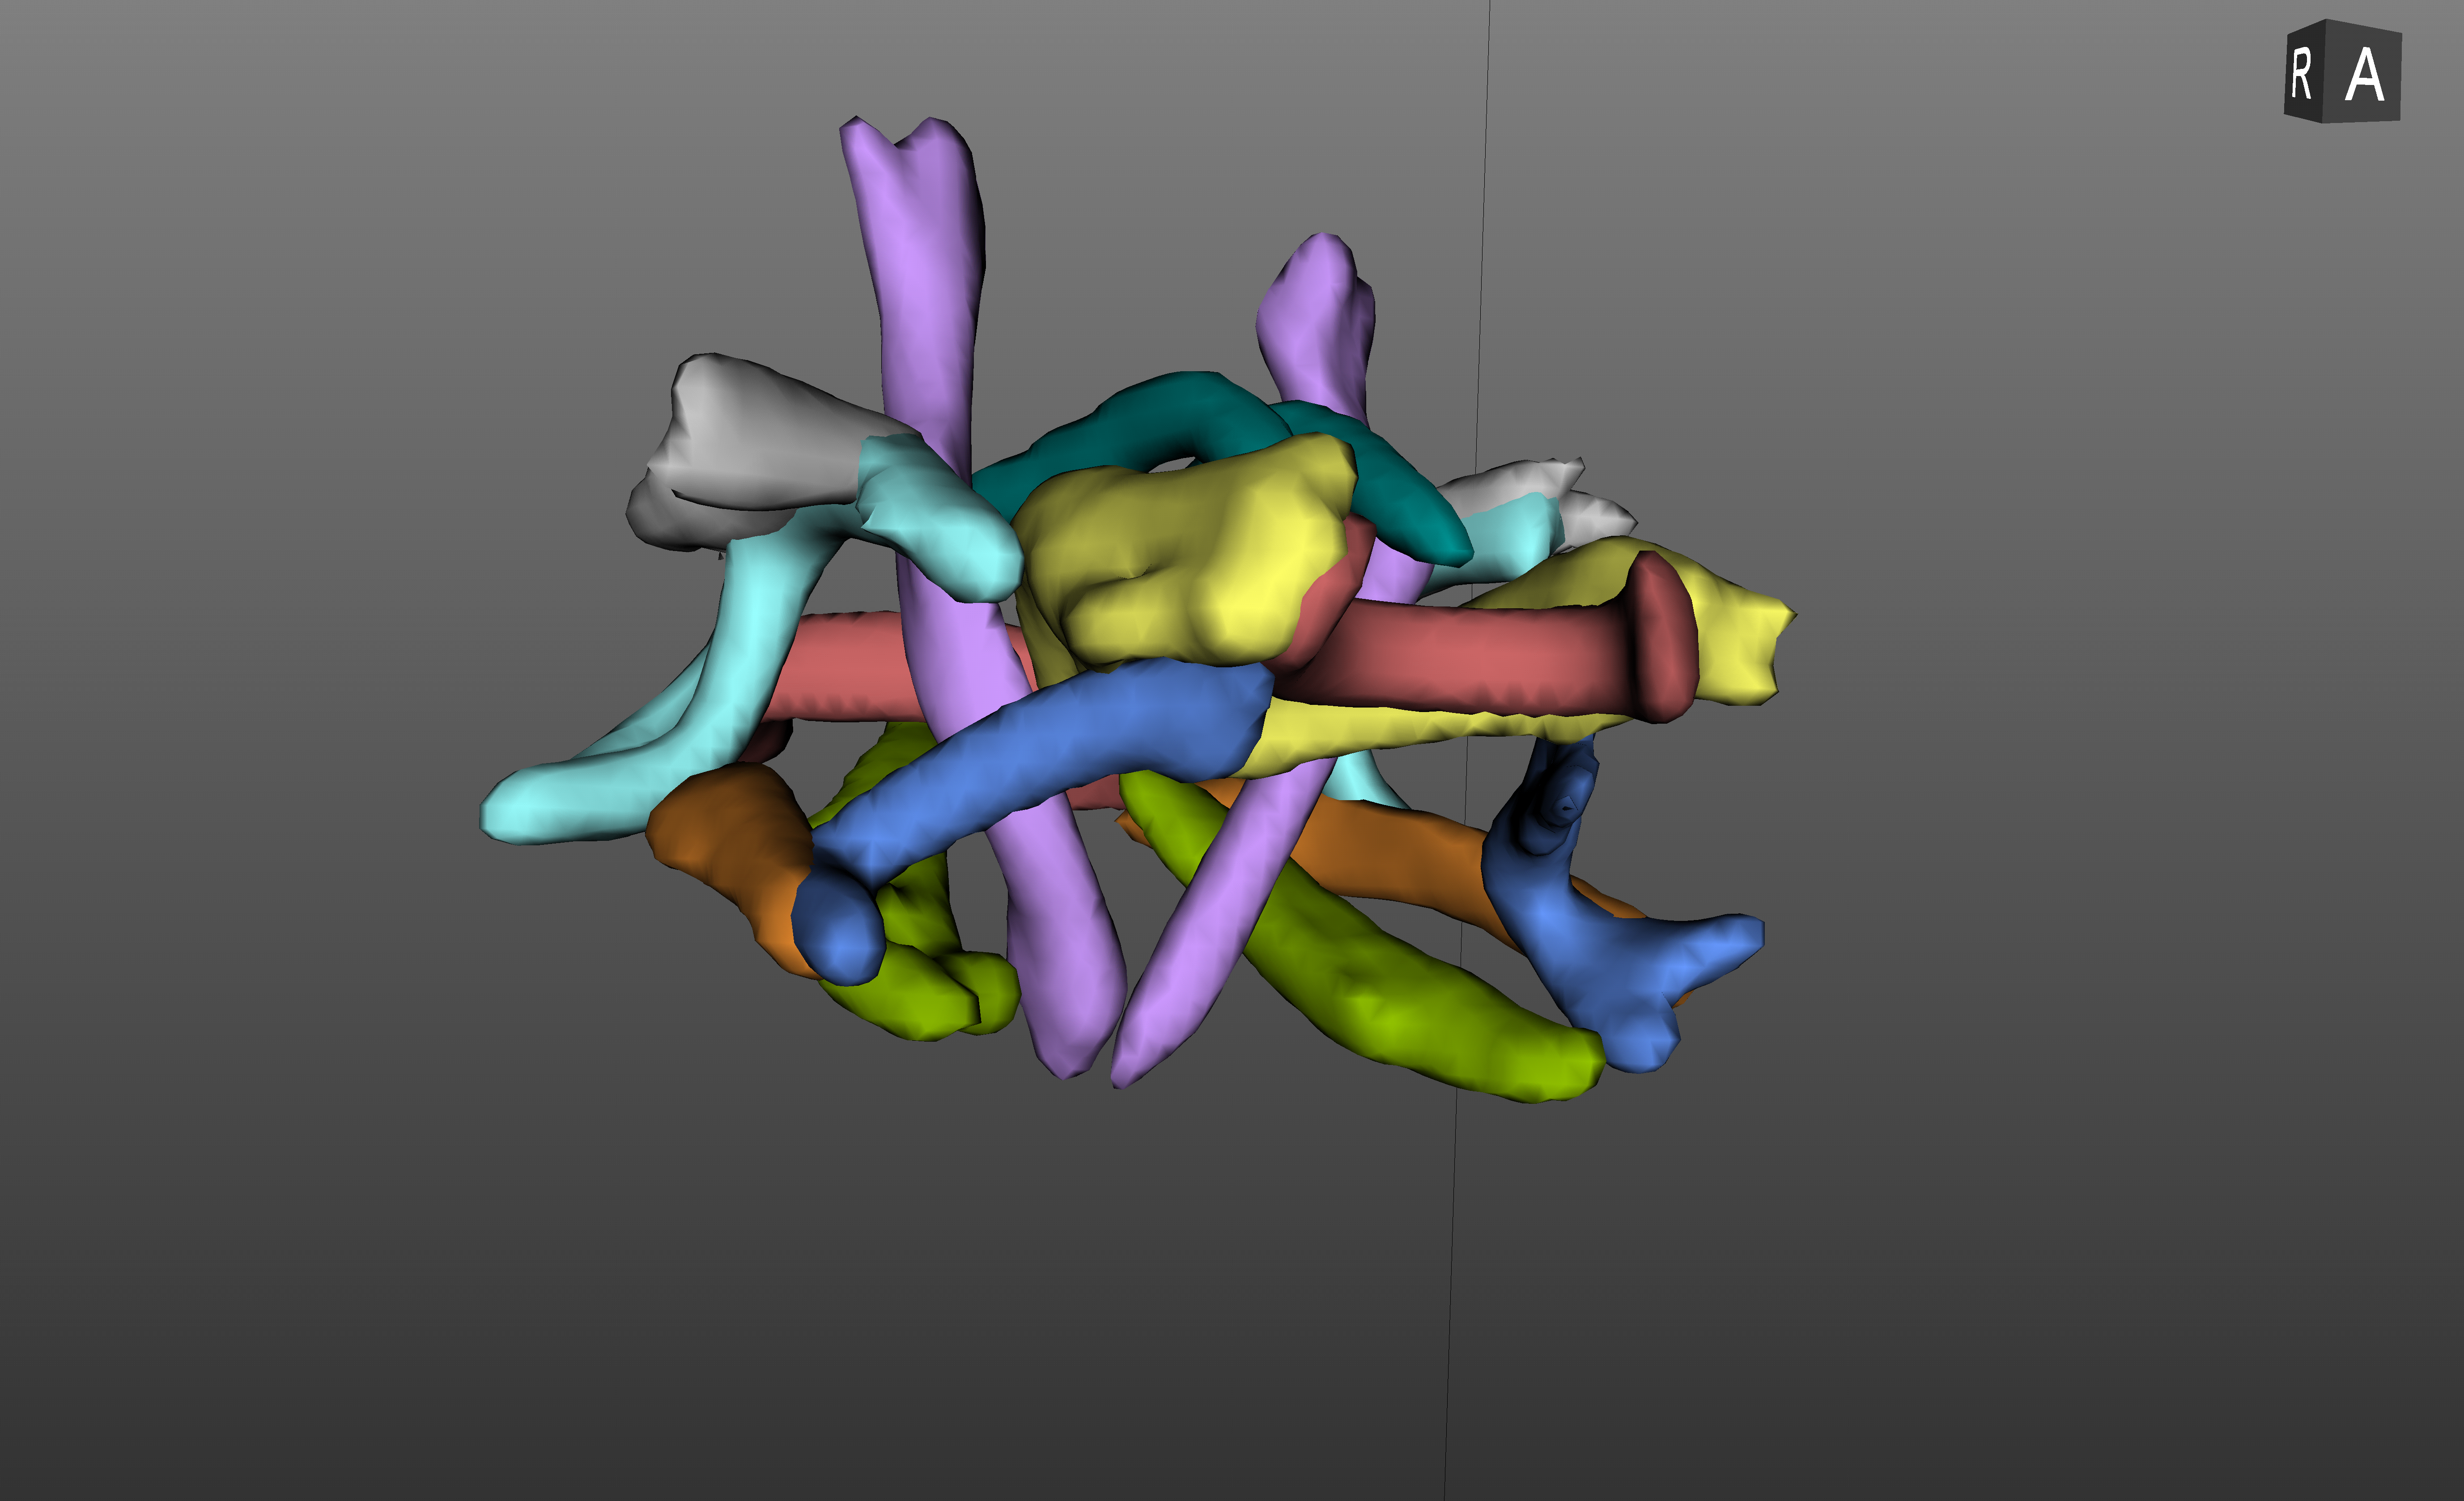
\includegraphics[width=\textwidth]{related/tracula}
				\caption{Probabilistic Tractography}
    \end{subfigure} 
    \caption{Full brain tractography}\label{fig_tracto_det_prob}
\end{figure}

\subsubsection{Tractography Clustering}

Another approach to simplify full brain tractography is by clustering it. This is more useful if the generated clusters match with true anatomical pathways.

\autocite{song_zhang_identifying_2008} explores two methods for clustering fiber bundles, in the first one, fibers are assigned to the same cluster if they are sufficiently close, while the second one tries to optimize a global measure of separation between clusters
\autocite{guevara_automatic_2012} presents a method based on an atlas composed of common pathways in a group of subjects, and manually labeled by experts. 
In \autocite{garyfallidis_dipy_2014} the \emph{quick bundles} is introduced. This algorithm is able to efficiently isolate fiber bundles that match known structures.

\subsubsection{Connectivity Networks}

Tractography can also be used to create brain networks where nodes are regions of interest and edges are defined by characteristics of the fibers that connect them. Recall that these networks can also be defined using fMRI data. Once these networks are constructed, methods from graph theory can be applied \autocite{rubinov_complex_2010}. For example it is possible to find well connected neighbours, find hubs, analyze the shortest path between nodes, and measure the mean degree of nodes.

\autocite{li_visual_2012} introduces a software for robust construction and analysis of brain networks in a group of subjects. In this software local diffusion or functional features are calculated at the position of each node, then the system tries to find the best position for the corresponding node in different subjects by minimizing the differences of these local features.
Visual techniques for comparing two weighted brain networks are studied in \autocite{alper_weighted_2013}. The tool is based on a research of common analysis tasks and interaction with domain experts. At the end, two visualizations are recommended based on a user study; one of them is based on node and links diagrams and performs well in small networks while the other one, based on a connectivity matrix, performs better in networks with many nodes and edges.


\subsection{Software for Visualization of Spatial Data}

Of course visualizing spatial data is one of the most important tasks in neuro-image research. It should be done at every step of the analysis, to verify quality, and make sure everything is going as expected, and so problems can be corrected opportunely.

As soon as the image is acquired it should be validated by the team that operates the MRI machine. This is usually done with proprietary software distributed by the scanner manufacturer. These systems can integrate processing algorithms as surface reconstructions or fiber tracking, and they can also provide advanced visualization options like 3D graphics and volume rendering.

%basic
% Osirix / PACS / Proprietary 
% MRICRON / ITKSNAP

After the files are downloaded from the scanner, they can be visualized by other members of the team in their own machines using open source software. A very powerful and popular choice is Osirix \autocite{rosset_osirix:_2004}, which provides several advanced visualization methods, and can be extended using plugins. Other light options are mricron and itk-snap. These packages also include tools for annotating images and performing manual and assisted segmentation of images.

%FSL-view \autocite{jenkinson_fsl_2012} 

Most of the processing packages described in this section also include visualization modules, for example \emph{FSL} includes a viewer called FSL-View which can display structural, diffusion and functional MRI data. 

%FreeView / TkView \autocite{fischl_freesurfer_2012} : Loading data from command line, specify the subject only once.

The \emph{FreeSurfer} package includes several visualization applications: FreeView, tkMedit, tkRegister and tkSurfer. These applications are tailored at the different stages of the FreeSurfer processing pipeline, including Tracula. tkSurfer specializes in visualization of cortical surface reconstructions together with scalar data (curvature, thickness, fMRI statistical maps, etc). TkMedit is designed for visualizing anatomical data, together with cortical surfaces and fMRI statistical maps which are added as overlays. This tool also provides mechanisms for drawing image segmentations. TkRegister is meant for controlling and correcting registration between images. Finally, FreeView is a full 3D viewer that can display cortical surfaces, tracula bundles, and images. It also provides mechanisms for comparing different subjects, for applying custom transformations, and for performing manual segmentation. A convenient feature from all FreeSurfer tools is that they can be launched and configured from the command line. If data is organized using the FreeSurfer subjects directory structure, the subject, images and surfaces can be specified by name in the command line. In this way it is easy to load several structures for a specific subject, and most importantly, repeating this view for several subjects. 

%SPM \autocite{friston_statistical_2006}

The SPM package also provides several options for visualizing data at every stage of the pipeline. Large portions of such pipeline rely on a correct registration between images, and fortunately SPM includes a very powerful visualization for verifying and correcting registration between images. The module for displaying results is also very powerful, and allows users to use different thresholds to filter results, find and display in a table activation peaks, and create 3D renders. It provides a \emph{glass brain} visualization, where three orthogonal slices are shown side by side, and activations from the whole volume are projected to these three planes. This provides a quick overview of the location of activations in the full volume, but is only effective if there are few activations. SPM also provides several views of the underlying statistical model, as contrasts and parameters estimates, and fitted and adjusted responses.

% BrainVisa \autocite{cointepas_brainvisa:_2001}

BrainVisa \autocite{cointepas_brainvisa:_2001} is a software that integrates data management, data processing and visualization. Raw data is loaded into a database and organized internally by the application, processing algorithms are executed by accessing data in this database, and results are stored in the same place. The user can select objects to visualize from the database, which at the end means that after loading raw data into the system the user won't have to worry about file locations of file formats any more. Unfortunately this package has not been upgraded since 2013.

% 3D Slicer \autocite{fedorov_3d_2012}

3D Slicer \autocite{fedorov_3d_2012} is a powerful applications that can display and manipulate several kinds of data. It has a plugins architecture, which allows developers from all around the world to add new functionality. This application can load and display all kinds of images, it can overlay two images together, do volume rendering and 3d reconstructions, it can perform semi-automatic segmentation, model reconstruction, and fiber tracking among others. 

% VTK / PARAVIEW \autocite{schroeder_design_1996} \autocite{ahrens_paraview:_2005}

Most of the applications mentioned above use VTK \autocite{schroeder_design_1996} for rendering. This is a high performance graphical library which implements several processing and visualization algorithms common in scientific visualizations. It includes modules for filtering, resampling and slicing volumes, it can perform volume rendering, it can calculate and display iso-contours from volume data, it can generate and display streamlines and apply color-maps and opacity to objects among other features. It also permits building interactive visualizations and linking several views together.
It is mature and has become standard for displaying and manipulating medical images. 

% Conclussion... why we need something else? why these are not appropriate for visual analytics or exploratory research?
Even though there are several options available for visualizing neuro-image based spatial data, they don't interact well with each other, and each of them seems to support  specific workflows. They were not designed for the highly iterative patterns common in exploratory analysis, and they are not easy to integrate with tabular data and related visualizations and analyzes. 

%---------------------------------------------------------------


%-------------------------------------------------------------------
%In \autocite{paus_mapping_2005} a meta study about brain development is presented. It makes the point that by looking at different modalities of information in an integrated way is useful for making better assessments of intersubjects variance. He also mentions the potential from alliances between image experts with social scientists, geneticists and mental health professionals.

%\autocite{lenroot_brain_2006} analyzes the development of adolescents brain based on about 4000 scans of 2000 subjects. It makes use of manual and automatic techniques for registration and segmentation.

%\autocite{konrad_vbmdti_2012} presents a study that integrates local diffusion and structural features from the Broca area to results in a verbal intelligence test. In their discussion they mention that it is hard to specify the direction of this relation, this is, if a the structural difference causes a difference in performance, or if learning of verbal skill causes a change at the structural level. 


\section{Visual Analytics for Brain Images}

% introduccion

The need for exploring and extracting knowledge from large data-sets has been recognized by several researchers and tools have been proposed to aid in this task, recognizing the necessity to link together spatial data with tabular data. 

For example, \autocite{steenwijk_integrated_2010} presents two integrated tools, one for processing of image data in order to extract features, and one for interactively visualization and exploration of such features. Data is visualized through scatter plots and parallel coordinates plots, using techniques such as brushing and coloring by a different variable.  Given one point in the exploration, the tool allows the user to find the raw data that originated it. The objective of these tools is generating hypotheses, and rapidly iterating through different features in order to find relationships with clinical outcomes. 

% coins \autocite{wood_harnessing_2014}
% xnat-soup \autocite{gutman_web_2014}

As of today, several neuro-science repositories are available, for example SPINE \autocite{guttmann_spine_2012}, LONI-IDA \autocite{van_horn_is_2009} and COINS \autocite{wood_harnessing_2014}. Through these repositories researchers who acquire large amount of data can share it with the broader community. Other researchers can request access to these data through the platform, and if granted, download the images and complementary data. As the amount of data available in these repositories grows larger, it becomes necessary to add advanced features to navigate through it and find the appropriate data for answering a specific question. The COINS system implemented a graphical query tool\autocite{wood_harnessing_2014} that lets researchers search for data by combining several types of filters in a graphical interface. The tool will display how much data is available at each branch of the query, and when the user is satisfied, it will assist in issuing the requests for access to the respective data owners.  After data access is granted, it can be downloaded.

Downloading data from these repositories creates a bottle-neck for users, therefore there are proposals to visualize and run analyzis on these data without the need to download it. In \autocite{gutman_web_2014} a web viewer for this data is presented. It includes a feature for sharing visualizations by sending a link to collaborators, which should make collaboration more efficient. It also includes a system for navigating by finding related data, and displaying it in a graph where each node is a subject. 

% content based search 
Another opportunity that emerges from these repositories is finding similar images based on the content of the images. This is, based on a similarity between the two images and not on associated variables. For example, \autocite{joshi_interactive_2009} presents a system that constantly indexes a repository in order to let researchers query the system for images similar to a given example. 

Invizian \autocite{bowman_query-based_2011, bowman_visual_2012, van_horn_graphical_2013} provides a representation of multiple brain scans in a ``Feature Similarity Space'', where brain surfaces are positioned in a 3d space in such a way that \emph{similar} brains are nearby. The similarity metric can be defined using scalar features calculated from each brain. The system integrates with ggobi to combine the spatial analysis with interactive analysis of scalar data using linked scatter plots, parallel coordinates visualizations, etc. It also provides mechanisms to filter the datasets in order to select or highlight specific subjects, which permits a rapid visual assessment of the correspondence between specific variables and the similarity space.  In \autocite{van_horn_graphical_2014} an extensive use case where the system is applied to the ADNI data-set is presented; relating the dementia diagnostic to several structural features like cortical thickness, cortical gray matter volume and cortical gray matter area. Note this system also integrates machine learning methods that can automatically find the best features to separate the data-set into specified groups. 

\bigskip
% conclussion
It can be seen that current advances in manipulation of structural brain data together with developments in visual analytics creates an opportunity for performing efficient data-driven analyzes of brain data. Current systems already permit some types of analyzes, but they are still limited specific kinds of data and workflows. This thesis proposes a model that, combined with user centered design, permits rapid implementation of custom applications that adjust to user needs and workflows. Moreover, the model is to designed to foster collaboration,so that derived applications can be integrated to perform more complex analyzes. This also creates an environment where multiple specialists can collaborate  efficiently, and where the research group can benefit directly from the work of each specialist. This is all directed towards making a better use of available data-sets to generate hypotheses and ultimately increase understanding of how the brain structure relates to its function. While the current project focuses on interactive visual analysis, it is designed to integrate automatic processing and data mining solutions to create a full visual analytics system.